\documentclass[../full_thesis/full_thesis.tex]{subfiles}

% Default image directory
\newcommand{\thisdir}{../glitches_in_CGW}
\graphicspath{{\thisdir/img/}}



\begin{document}


Continuous gravitational waves from neutron stars could provide an invaluable
resource to learn about their interior physics. One common detection method involves
matched filtering a modelled template against the noisy gravitational wave data
to find unknown signals. As introduced in Chapter~\ref{sec: intro to cgw}, this
method suffers a mismatch (a loss of signal to noise ratio) if the unknown
signal deviates from the template. One significant way this may happen is if
the neutron star undergoes a glitch, a sudden rapid increase in the rotation
frequency as introduced in Section~\ref{sec: glitches}, a phenomenon seen in the
timing of many radio pulsars.  While the mechanism which causes pulsars to
glitch is not fully understood, it is likely that any continuous
gravitational waves emitted by the star will also be affected by the glitch since
both are intimately related to the neutron star crust.

In this chapter, we use information on the rate and size of pulsar glitches, as
deduced from the observed population of glitching radio pulsars, to estimate
the potential mismatch introduced when searching for gravitational waves from
neutron stars whose rotational timing is unknown. We intend to publish this
chapter, along with the generalised mismatch defined in Sec.~\ref{sec:
generalising the metric-mismatch}, in due course.

 %This includes blind all-sky gravitational wave searches for completely
 %unknown neutron stars, and also directed searches on smaller high interest
 %regions, e.g. supernova remnants, or the Galactic centre.
% We assume the gravitational waves are emitted at twice the rotation frequency,
%as is appropriate for a rigidly rotating, steadily spinning star. We find
%that for conservative estimates, neutron stars in large portions of the
%parameter space searched in all-sky gravitational wave searches will glitch
%during the search with a magnitude that will render the signal lost in
%fully-coherent follow-ups.


\section{Introduction}
\label{sec: glitches introduction}

Electromagnetic (EM) observations of pulsar glitches have long been one of the most
fruitful sources of insight into neutron star physics. Glitches are characterised
by a sudden increase in the rotation frequency, often accompanied by a jump in
the frequency derivative and an exponential recovery of some fraction of the
initial frequency jump. The events happen
rapidly and are sufficiently disruptive that pulsar timing models often loose phase
coherence over the event.

Two leading models exist to explain glitches. In the \emph{superfluid pinning}
model, some portion of the interior superfluid is pinned, and does not
participate in the smooth torque-driven spin-down of the rest of the
crust (where `crust' refers to the actual crust, plus whatever other parts of
the star that are strongly coupled to it).  After some period, the crust will
therefore have developed a frequency lag compared to the pinned superfluid. A
glitch occurs when the two components recouple, transferring
angular momentum from the pinned superfluid to the crust and producing a
spin-up of the crust \citep{Anderson1975, Alpar1984}.  Alternatively glitches
could be caused by \emph{crust cracking} as the crust readjusts to a minimum
energy configuration brought about by the gradual decay of the spin-down rate
\citep{Baym1971}.  It is also possible that glitches result from a combination
of these two models; evidence for this was found by \citet{Melatos2008}.  In
either case it seems reasonable to assume that both the crust and the core will
be involved.

Rotating isolated neutron stars can produce continuous gravitational-wave (GW)
emission from non-axisymmetric distortions, colloquially also known as `mountains'. These
require the mountain to be supported by either elastic stresses in the crust or
magnetic fields. In this model, the star emits a monochromatic GW at a
frequency $\nuS$ which is twice the rotation frequency $\nuS$, i.e, $\nuS=2\nuR$.

It is unclear exactly how a glitch, as observed in the EM channel, will
manifest in the GW channel.  Observing a glitch in both the EM and GW channels
would provide a unique opportunity to investigate the neutron star interior, but to do
this we must first detect continuous GW emission.

Estimates for the intrinsic gravitational wave strain amplitude
$h_0$ for canonical models of GW emissions (see for example \citet{abbott2008beating})
suggest they are extremely weak compared to the noise level of advanced
detectors \citep{aasi2015narrow}.  As a result, in order to detect a signal,
significant effort has been put into advanced data analysis methods,
which may be capable of identifying the putative signals. Many of these methods
rely on \emph{matched filtering} in which a template is correlated with the data
with the hope of detecting the presence of the unknown signal similar to the
template. The power of these methods is that
the signal-to-noise ratio (SNR) scales as the square-root of the observation
time \citep{Prix2009}. Due to the longevity of GW signals, this allows the weak
signal to be discerned from the noise.

These methods are powerful, but harbour a vulnerability in any instance where
the template, a Taylor expansion in the phase usually up to second order, does
not match the signal. For GW signals from non-axisymmetric distortions of neutron stars,
we can expect that discrepancies from such a template may manifest in one of
two ways. Firstly, we know from radio pulsar timing that the spin-down of a pulsar
differs from a Taylor expansion due to timing noise. We will
consider the effect of timing noise in Chapter~\ref{sec: timing noise in cgw}
and Chapter~\ref{sec: timing noise in cgw analytic};
%This is
%continuous low-frequency structure in the residual between the best-fit Taylor
%expansion timing model and the observed pulsations; for a review see
%\citet{Hobbs2010}. The effect of timing noise on continuous GW searches was
%first studied by \citet{Jones2004}. When performing a targeted search for a
%known radio pulsar, \citet{Pitkin2004} developed a method to include the
%contribution of timing noise, as seen in the EM channel, into the GW template. In
%\citet{Ashton2015} we have previously used the Crab pulsar to estimate the
%effect of timing noise for fully-coherent searches. 
in this chapter we will
address the second potential manifestation: glitches.

There are two distinct questions to answer in the case of glitches: `how
probable is it that a glitch will occur during our GW observation?', and `if a
glitch does occur, what effect will it have on our ability to discover the GW
signal?'. To answer these questions, we first use known radio pulsar glitch
statistics to estimate the size and rate of radio pulsar glitches for the
parameter spaces considered in continuous GW searches. Then, we assume that the
EM and GW channels are locked in phase, such that a glitch observed in radio
pulsations also exist in the GW signal at twice the phase, frequency and
spin-down rate. Having obtained an estimate for the magnitude and rate of glitches
for potential continuous GW sources, we quantify the effect such glitches will
have on current continuous GW detection methods by calculating the mismatch. We
will do this using the generalised metric-mismatch introduced in Section~\ref{sec:
generalising the metric-mismatch}. Specifically, we model a glitch as a
piecewise Taylor expansion with a discontinuity at the glitch; we do not model
the exponential recovery observed in some glitches, but we will discuss the
significance this may have in Section~\ref{sec: recovery}. Ultimately, the goal of
this chapter is to estimate the risk faced by current and ongoing continuous GW
searches to glitches in their target population.

%We can distinguish between two types of GW search: those where we know the
%timing properties, and hence if the source has undergone a glitch, and those
%which we dont. The first type are known as \emph{targetted} when a search is
%performed for GWs from a known radio pulsar, in this search the sky location
%and timing properties can be estimated from the radio pulsations. The second
%type include both \emph{directed} searches, where the sky location is known,
%but not the timing properties as in a search for GWs from supernova remnants,
%and \emph{all-sky} searches in which we blindly search for signals from any
%location. It is the second type of GW searches that, if the search assumes
%there is no glitch, are most at risk from glitches.

The remainder of this chapter is organised in the following way. We begin in
Section~\ref{sec: continuous gravitational-wave searches}, with a description
of current GW searches and how glitches may effect them. Then, in
Section~\ref{sec: statistical properties} we investigate the statistical
properties of the observed radio pulsar glitches. In Section~\ref{sec: mismatch
due to glitches} we calculate, given the properties of a single glitch, the
corresponding mismatch for a semi-coherent and fully-coherent search.  To give
quantitative results relevant to real GW searches, in Section~\ref{sec:
estimating the mismatch} we use these calculations to transform the predicted
glitch sizes into predicted mismatches and rates for GW searches.

\section{Continuous gravitational-wave searches}
\label{sec: continuous gravitational-wave searches}

Searches which target a particular source making use of the EM emission (for
example the \citet{abbott2010searches} targeted search for the Crab pulsar) are able to
handle the epoch of a glitch, either by avoiding searches over the glitch, or
allowing for a jump in the timing solution at that point \citep{abbott2010searches}. By
this merit, such searches have a very low risk of being disrupted by a glitch
coupled to the EM channel, provided the GW channel follows closely the phase
evolution of the EM channel.

In contrast, blind GW searches which, by definition, search for signals without an
EM counterpart do not have any such prior knowledge. This category of searches
includes both \emph{directed} searches where a small patch of sky is searched
in which a neutron star is believed to exist (e.g. the \citet{aasi2015searches} search
for continuous GWs from supernova remnants), and \emph{all-sky} searches; in
both instances a band of frequencies and frequency-derivatives are usually
searched since they are inherently unknown. Typically, these searches
match filter against smooth templates built from a Taylor expansion in
the phase; as such the templates do not include glitches. If a neutron star, emitting
detectable levels of GW emission, undergoes a glitch in the GW channel, then the
matched filtering method may fail because the template is a poor match to the
real, glitching signal.

All-sky and targeted blind searches are most notably at risk of glitch
disruption and so it is these which we fill focus on in this chapter. Continuous GW searches ideally employ a
\emph{fully-coherent} search which consists of matched filtering the template
against the data over a coherence time $\Tcoh$.  However, such a search is
computationally intensive and so GW searches typically revert to using a
\emph{semi-coherent} method in which the total observation time $\Tspan$ is
divided into $\Nseg$ segments each of duration $\Tcoh$. Each of these is then
fully-coherently searched and then recombined to give a semi-coherent
measurement which is insensitive to phase jumps between segments. This method
provides more sensitive searches at fixed computing cost \citep{Prix2012}.
Typically, a semi-coherent search is performed first,
then interesting candidates are \emph{followed-up}, reducing the number of
segments, aiming to finally detect the signal with a fully-coherent search;
see \citet{Shaltev2013} for a two-stage follow-up procedure.

A variety of targeted and all-sky searches have already been completed, with
more ongoing and planned for the advanced detector era. In Table~\ref{tab: searches}
we list the search parameters used in some recent searches.
\begin{table}[htb]
\centering
\footnotesize
\begin{tabular}{l|c|c|c|c|c|c}
 & $\nuS$ & $\nudotS$ & $\Tcoh$ & $\Tspan$ & Ref \\
 & [Hz] & [nHz/s] & [hrs] & [days] & \\ \hline
S5 E@H all-sky & 50, 1190 & -2, 0.1 & 25 & 694 &  \citep{aasi2013einstein}\\
%S5 E@H galactic center & [1250, 1500] & [-2.93, 0.553] & 25 & 653.18 &  \citep{}\\
S5 E@H galactic center & 78, 496 & -71, 0 & 11.5 & 302 &  \citep{aasi2013directed}\\
%S6 all-sky bucket & 50, 452 & -2.6, 0.3 & 60 & 255 &  \citep{}\\
S5 all-sky & 50, 1000 & -0.89, 0 & 0.5 & 365 & \citep{aasi2014application} \\
VSR low-freq. all-sky & 20, 128 & -10, 0.15 & 2.3 & 185 & \citep{aasi2016first}\\
S5 supernova remnant (Cas A) & 91, 573 & -60.5, -1.6 & N/A & 8.4 & \citep{aasi2015searches} \\
%O1 E@H all-sky & 20, 100 & -2.6, 0.26 & 210 & 180? & \citep{}

\end{tabular}
\caption{Summary of some recent all-sky and directed searches. All numbers are
approximate, see the references for exact ranges. Note that S5
refers to data from the fifth LIGO science run, similarly VSR
refers to data from the second and fourth Virgo science runs. For the S5 supernova
remnant search we present parameters for the Cassiopeia A search only and note that
this was a fully-coherent search with no semi-coherent stage.}
\label{tab: searches}
\end{table}

To make practical use of the results obtained in this chapter, we will make
predictions for the glitch rate and magnitude in the context of typical GW
searches. As an illustrative example, we will use the search parameters that
were used in LIGO's Einstein@Home all-sky search for periodic gravitational waves
in the fifth science run (S5) data \citep{aasi2013einstein}, hereafter referred to
as the E@H search. This search used the semi-coherent \emph{Hough-transform}
method \citep{Krishnan2004} and is typical in terms of the timing parameters,
although in future searches it is expected that the number of segments will be
decreased due to improvements in computing power.  We find in Section~\ref{sec:
mismatch due to glitches} that the effect of a glitch is independent of the
sign of the frequency derivative, and so for convenience we truncate the GW
spin-down parameter space to $\nudotS = [-2, 0]\times10^{-9}$~Hz~s$^{-1}$.


\section{Statistical properties of the observed glitch database}
\label{sec: statistical properties}
In this section, we will discuss the properties of glitches in the observed
radio pulsar population using the glitch catalogue maintained by \citet{Espinoza2011}
and available at \url{www.jb.man.ac.uk/pulsar/glitches.html}.
Our goal is to make a statement about how often glitches occur and their
magnitudes for the types of neutron star which may be emitting GWs in the
parameter space of typical GW searches.  This task is made difficult since many
searches look for young, rapidly rotating stars for which we only have a small
sample of observations. Therefore, we must moderately extrapolate to apply our
results to the observed radio pulsar population.

Radio pulsar timing methods detect glitches by fitting a piecewise Taylor
expansion in the phase on either side of the event, with a modelled jump in
between (see \citet{Edwards2006} or Section~\ref{sec: glitches} for a detailed
discussion). The glitch catalogue reports 472 events from
165 pulsars (as of the 27$^{\rm th}$ of June 2016); for each of these events a
value is reported for the frequency jump $\DnuRglitch$ and frequency derivative
$\DnudotRglitch$, if it can be measured. We cross-reference the glitch
catalogue with the ATNF \citet{ATNF} pulsar catalogue available at
\url{www.atnf.csiro.au/people/pulsar/psrcat/} in order to get the glitching
pulsar's timing properties.

Of the 472 listed glitches, we find 15 with no ATNF cross-reference, 1 with
$\DnuRglitch < 0$, and 4 with no measured $\nudotR$ in the ATNF catalogue; these
pulsars are removed from our data set. Additionally, we find 54 glitches which
have either no measured $\DnudotRglitch$, or a measured value consistent with 0.
These will be included where possible.

\subsection{Glitch magnitudes}
\label{sec: observed glitch magnitude}

\citet{Espinoza2011} argued that the glitch catalogue contains glitches from
two distinct sub-populations of pulsars. There is the main population with
$\DnuRglitch$ magnitudes ranging from $10^{-9}$ to $10^{-5}$~Hz, and a second,
less numerous population with larger magnitudes of $\DnuRglitch$. The smaller
population are described as `Vela-like' in that the pulsars that undergo these
glitches have similar
characteristic ages and magnetic fields to the Vela pulsar (B0833-45).  We reproduce the evidence for this finding in
Figure~\ref{fig: Delta nu mixture} where we plot the histogram of all observed
$\DnuRglitch$ values. This demonstrates the bimodality found by \citet{Espinoza2011}.

To check that the bimodality is not an artefact of the histogram bin sizes we
estimate the probability density function using a Gaussian kernel density
estimate (KDE). Specifically we use the \citet*{Scipy} implementation. This is
also plotted in Figure~\ref{fig: Delta nu mixture} and demonstrates two distinct
peaks, although the smaller peak could be interpreted as two modes close together.

By eye, it is clear that there are at least two modes to the histogram. However,
it is also possible that there may be more modes with less distinct differences
in their mean. We investigate this issue in Appendix~\ref{sec: Bayesian model
comparison} by applying a Bayesian model comparison to Gaussian
mixture models (see
Chapter~18 of \citet{gelman2013bayesian} for an introduction to mixture models) varying the number of components and also allowing for a skew as
described in \citet{Ohagan1976}.  We find that all models with 2 or more
components fit the data decisively better than a single component. Marginal
gains are found by allowing the models to be skewed and have 4 or more
components, but no single model is outstanding amongst the others. For this
reason we choose to use a 2-component model with skew; this provides a good
empirical description of the data and is pragmatic in that we limit the number
of components to 2 for interpretability. We note that this description is
empirical and we do not intend to make any substantive claim relating the two
components to the two mechanisms discussed in Chapter~\ref{sec: glitches}.

Having obtained a fit to the magnitude of the glitch in frequency using a
2-component skewed-Gaussian mixture model, we use this fit to label each data
point as originating from one of the 2 skewed-Gaussian components . Specifically, to
each data point we assign the label based on the maximum probabilities of each
of the two components, given the maximum posterior model parameters derived in
the fitting process.

The resulting mixture components and individual
distributions are plotted in Figure~\ref{fig: Delta nu mixture} and in
Table~\ref{tab: mixture components} we provide the resulting mean, standard
deviation, weights and skewness of the two components in log-space.
This method identifies the two subpopulations in a manner consistent with the
observations by \citet{Espinoza2011} and notably the Vela-like component suffers
a significant skew.

\begin{table}[htb]
\begin{tabular}{lcccc}
& Mean &Std. Dev. & Weight & Skew \\ \hline
Normal & -8.413 & 1.590 & 0.701 & 1.084 \\ 
Vela-like & -4.407 & 0.534 & 0.299 & -9.660
\end{tabular}
\caption{Log-normal mean, standard deviation and weight for the components of
the mixture model as fitted in Figure~\ref{fig: Delta nu mixture}.}
\label{tab: mixture components}
\end{table}

\begin{figure}[htb]
\centering
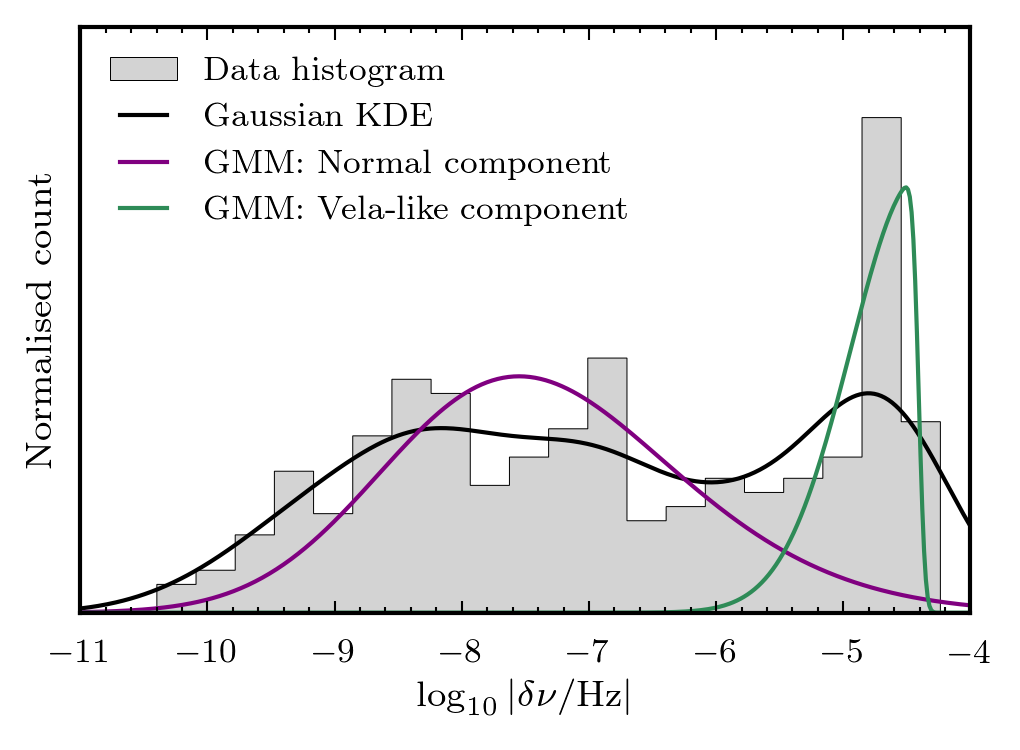
\includegraphics[]{MixtureModel_for_DeltaF}
\caption{The distribution of glitch magnitudes $\DnuRglitch$ observed in the
glitch catalogue. This is given as both a binned histogram and a Gaussian
KDE, as discussed in the text. The coloured lines mark the two components of
the skewed Gaussian mixture model fitted to model the bimodality.}
\label{fig: Delta nu mixture}
\end{figure}

In Figure~\ref{fig: Espinoza dF dF1}, we plot histograms for $\DnuRglitch$ and
$\DnudotRglitch$ along with the raw data in a scatter plot. We have separated
the data into the individual sub-populations, as labelled by the Gaussian
mixture model, and colour coded to aid the eye. Several pulsars of interest are
picked out using coloured halos. It is of general interest that not all the
Vela glitches are categorised by our method as Vela-like; this can be seen by
looking at the distribution of Vela glitches in Figure~\ref{fig:
Espinoza dF dF1}.
\begin{figure*}[htb]
\centering
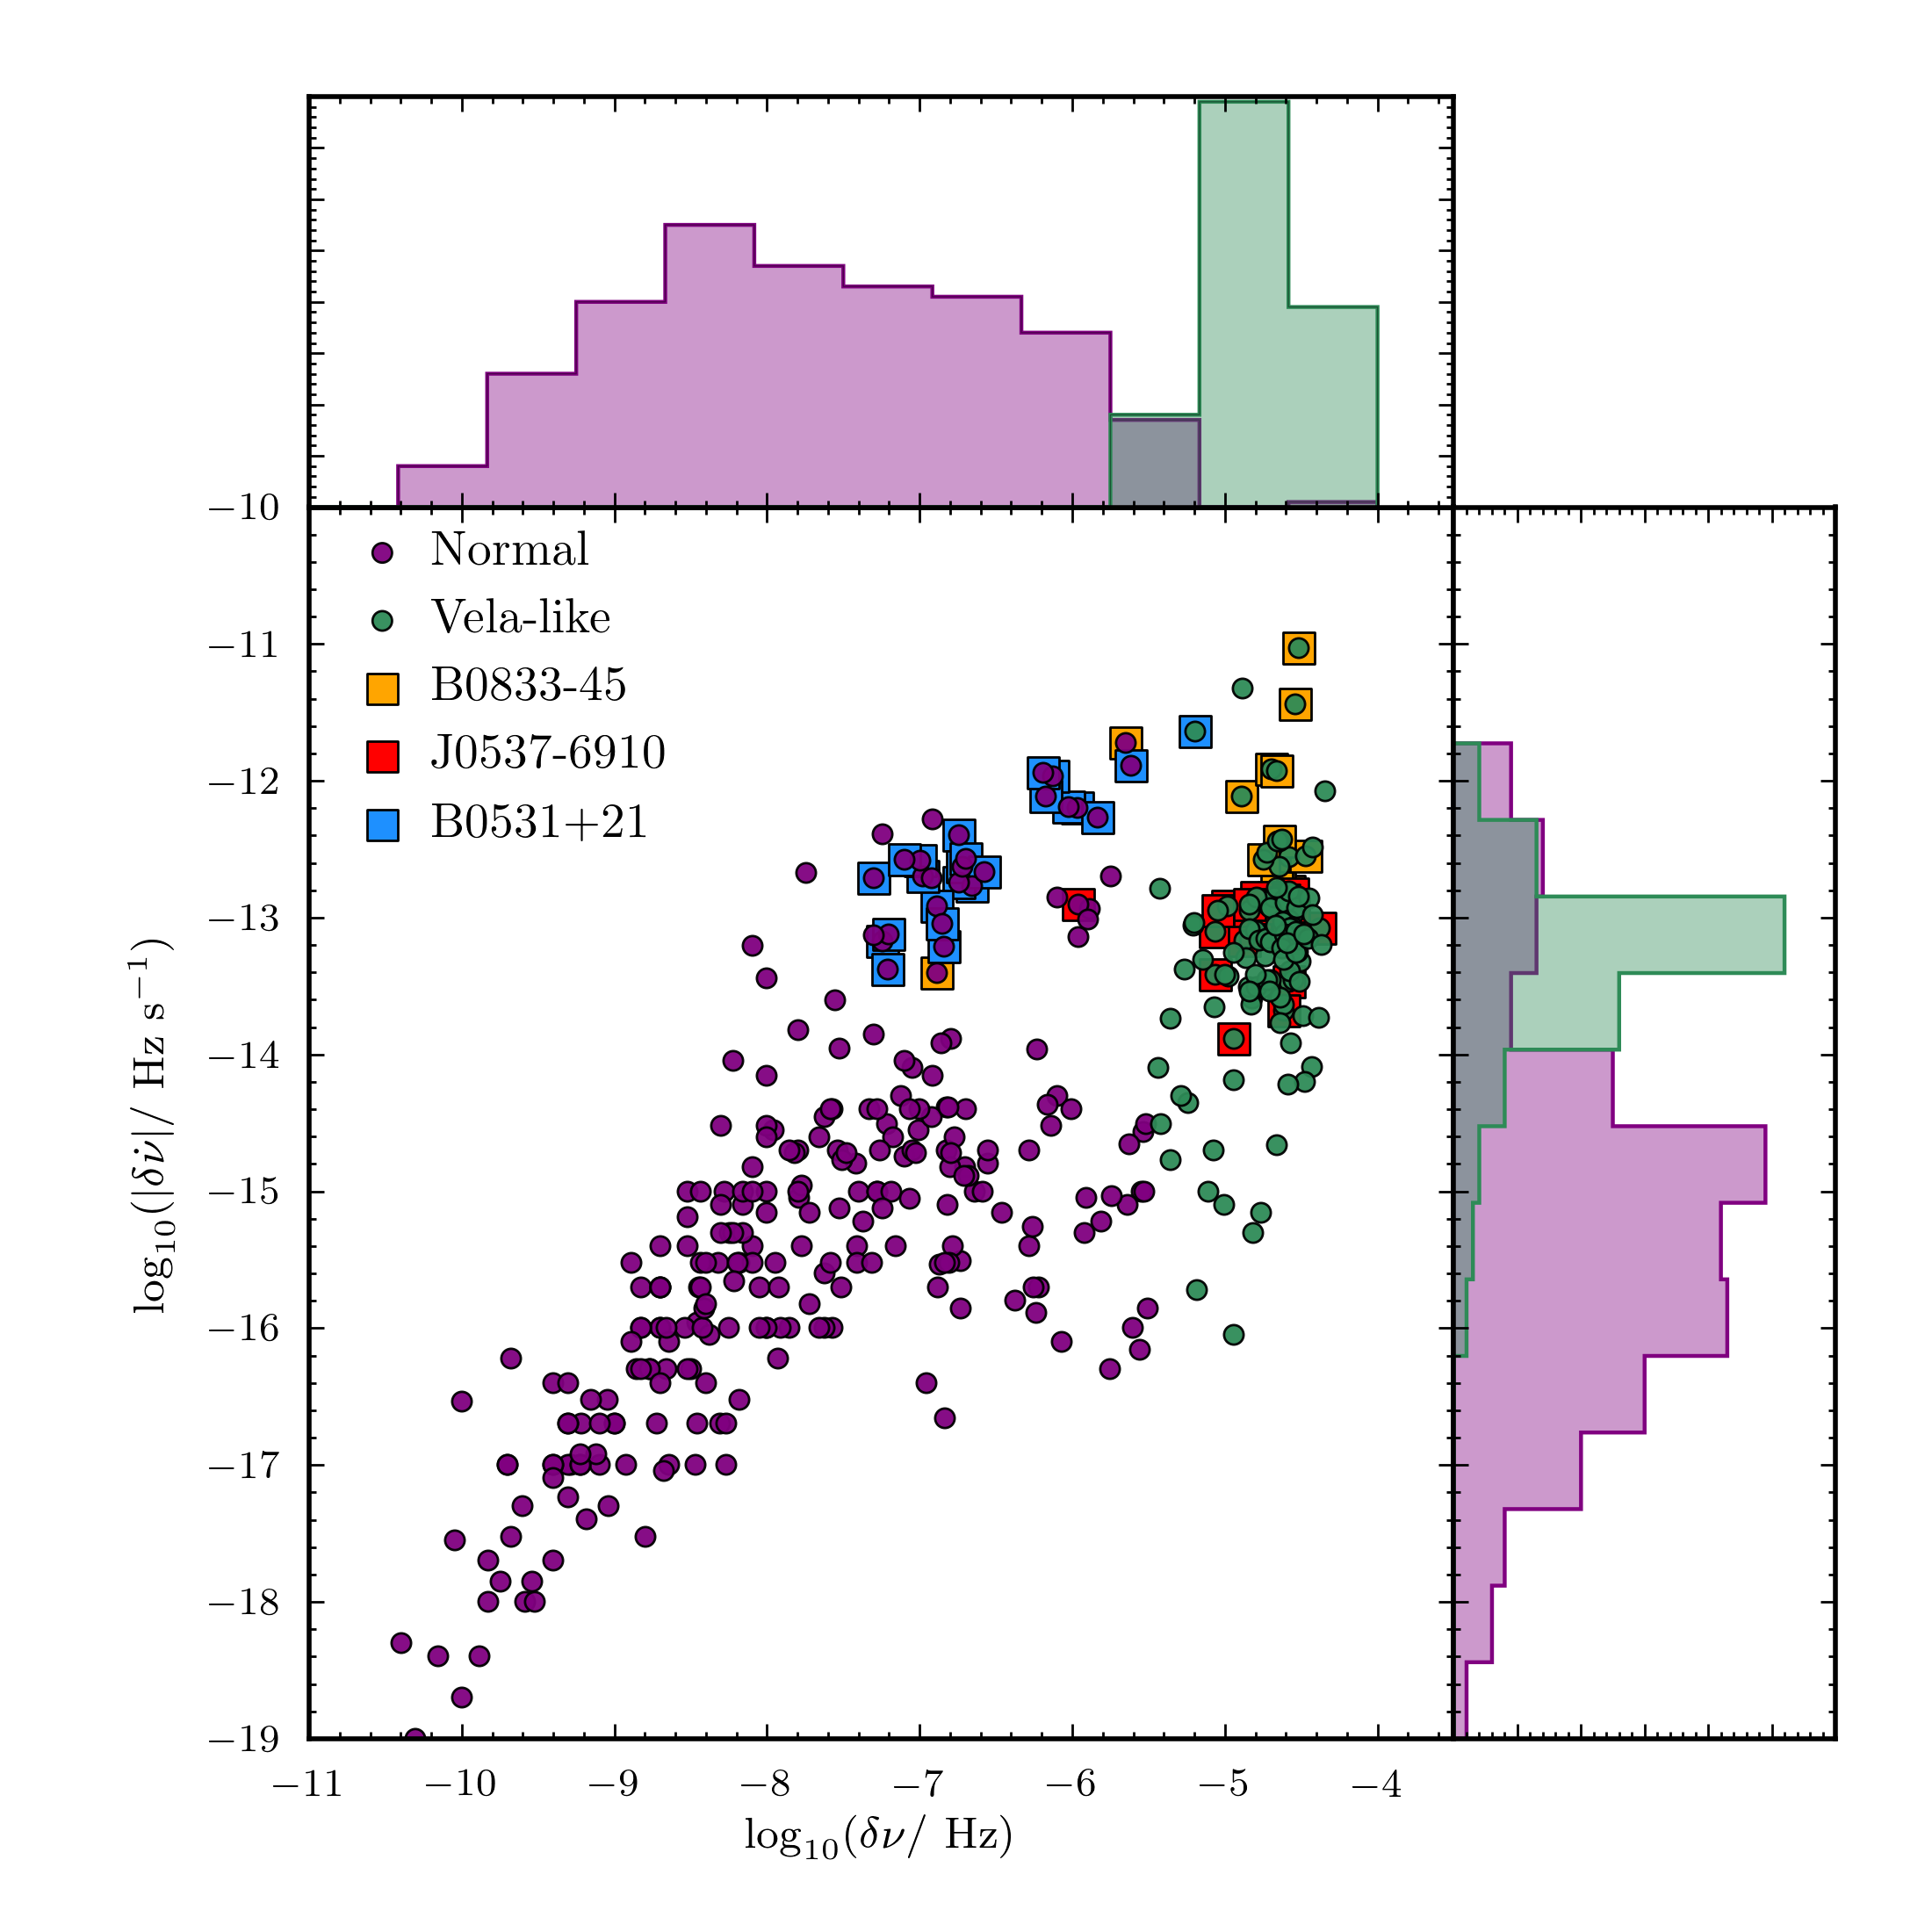
\includegraphics[width=0.75\textwidth]{Combined_dF_dF1}
\caption{Glitch magnitudes as provided by the glitch-database
         \citep{Espinoza2011}. This shows a scatter plot of all pairs of
         $\DnuRglitch$ and $\DnudotRglitch$ where the colouring depends on the
         labelling given by the mixture model. Purple circles are the
         points categorised as `normal glitches', while green
         circles are the points from the `Vela-like' population. Histograms for
         both glitch magnitudes are also given for each sub-population.
         Coloured halos highlight glitches from interesting pulsars.}
\label{fig: Espinoza dF dF1}
\end{figure*}

%The bimodality labelled by the Gaussian mixture model,
%which was conditioned only on the $\DnuRglitch$ data, is also visible in the
%$\DnudotRglitch$ data. Alternatively we could have conditioned on both data sets:
%this was tried and led to a looser clustering which did not pick out the tight
%bundle of Vela-like glitches.

\subsection{Overview of the population of glitches}
\label{sec: overview of the population of glitches}


To give an overview of all observed glitches in the context of the whole population of
observed radio pulsars listed in the ATNF catalogue, in Figure~\ref{fig: nu
nudot} we plot two copies of the familiar $\nuR$-$\nudotR$ diagram. In panel A, for each
pulsar which has been observed to glitch we add a coloured circle. Those
pulsars which glitched multiple times are marked by a larger coloured circle
with the area proportional to the number of glitches. In panel B, we again mark
each pulsar that has been observed to glitch with a coloured circle, but here
the area of the coloured halo marks the pulsar's average glitch magnitude.
For both plots, different
colours have been used to partition the Vela-like and normal glitches (note that some
pulsars display glitches from both populations) and a shaded box marks the
parameter space searched by the S5 E@H search. Finally, dashed lines mark isoclines
of constant characteristic age as defined by $\tauAge = \left|\nuR/\nudotR\right|$.
\begin{figure}[htb]
\centering
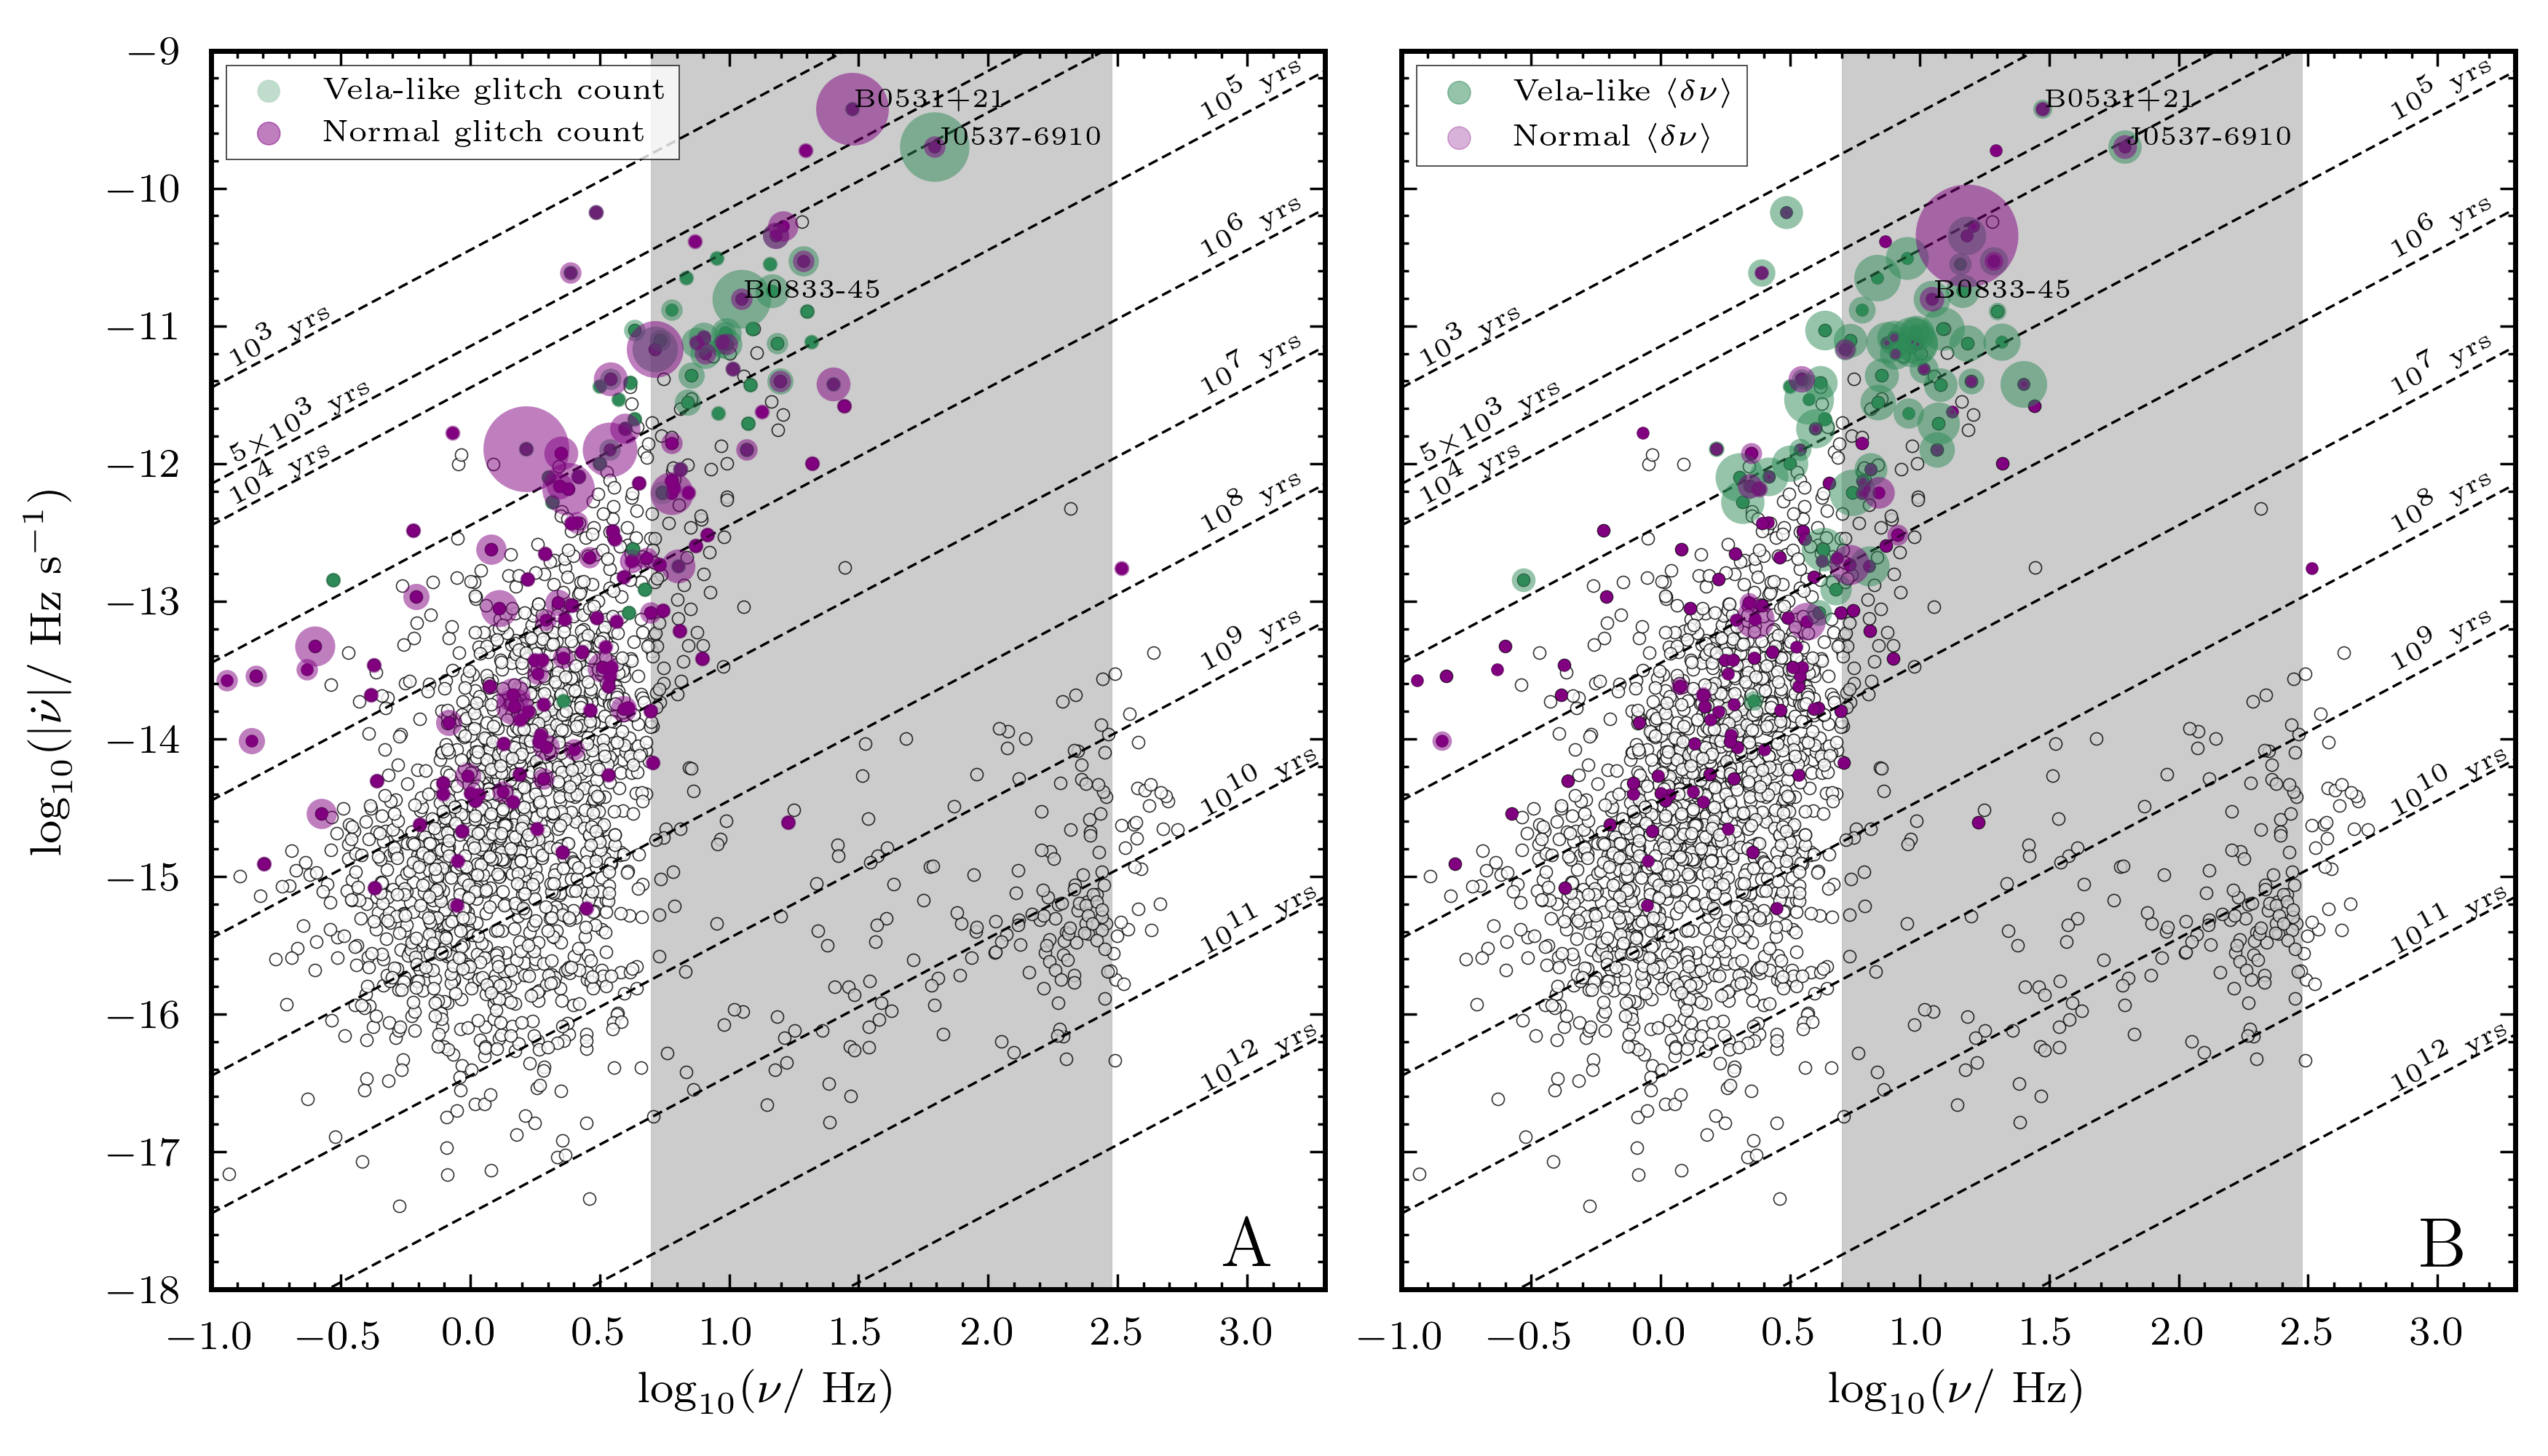
\includegraphics[width=\textwidth]{nu_nudot}
\caption{Frequency-frequency derivative plot of all pulsars in the ATNF
catalogue \citep{ATNF}. \textbf{A}: A single coloured point marks pulsars which have been
observed to glitch; the area of the coloured halo is proportional to the
number of observed glitches from that pulsar. \textbf{B}: A single coloured
point marks pulsars which have been observed to glitch, the area of the coloured
halo is proportional to the average glitch magnitude from that pulsar. We have used
purple for `normal' glitches and green for `Vela-like` glitches, as defined by
the skewed Gaussian mixture model in Section~\ref{sec: observed glitch magnitude}. Note
that, for the glitch magnitudes, the relative scaling for the Vela-like and
normal populations are \emph{not}
the same since the Vela-like pulsars are significantly larger: the area representing
the normal glitch magnitudes are scaled 3 times larger than the Vela-like glitch
magnitudes.
The gray shaded box marks the parameter space of typical GW all-sky searches which
cover a rotational frequency $\nuR$ range of $10-600$ Hz (assuming they search for signals
with $\nuS=2\nuS$).}
\label{fig: nu nudot}
\end{figure}

While the bulk of observed glitching pulsars are from the main pulsar population, the
fraction of young pulsars ($\tauAge < 10^{5}$~yrs) which glitch is proportionally
higher than in the normal population. Vela-like glitches occur predominantly
in the young pulsars with none seen in pulsars with $\tauAge > 10^{7}$~yrs. It
is also noticeable that younger pulsars display a greater number of glitches. Note
that, since we have not observed all pulsars
for the same duration, one cannot infer the relative glitch rate from the
number of glitches alone.

%The S5 E@H search space spans all observed spin-down rates; however, the discretisation
%is done linearly. The population of old pulsars with large frequencies, but small
%$\nudotR$ values which lie in the E@H parameter space are the
%so-called millisecond pulsars \citet{Lyne1988}; these are not targeted by the E@H search.

For the normal-glitch population, \citet{Espinoza2011} noted that pulsars with
$\tauAge < 5\times10^{3} $~yr undergo small or medium sized glitches
($\DnuRglitch < 10^{5}$~Hz).  It is postulated that the higher temperatures in
younger pulsars prevents the glitch mechanism working effectively. This effect
is consistent with Figure~\ref{fig: nu nudot}B: the pulsars with the largest
average glitch sizes have $\tauAge \sim 10^{5}$~yrs, while younger pulsars tend
to exhibit smaller glitches on average.

\subsection{Extrapolating: glitch magnitudes}

We would like to be able to predict the glitch magnitude for the unobserved
pulsar population targeted by GW searches. In particular, we need to
extrapolate up to the large values of $\nudotR$ searched for in many all-sky
GW searches, where few observed radio pulsars exist.

It has previously been found by \citet{Mckenna1990}, \citet{Lyne2000},
\citet{Wang2000}, and \citet{Espinoza2011}
that the glitch activity (defined in the first of these references) correlates
well with $|\nudotR|$ and the characteristic age
$\tauAge$. We choose not to combine the rate and
magnitude information together into the activity, but estimate both separately
as these are of most direct relevance to GW searches.

We investigated correlations of the
glitch magnitudes $\DnuRglitch$ and $\DnudotRglitch$ with the frequency,
frequency-derivative and characteristic age.
In Table~\ref{tab: correlation} we present the Pearson correlation coefficient
for each glitch magnitude ($\DnuRglitch$ and $\DnudotRglitch$).
This is done for three groups:
all the data together, then individually for the normal population and the
Vela-like population.
\begin{table}[htb]
\begin{tabular}{l|l|ccc}
&  & $\log_{10}|\tauAge|$ & $\log_{10}|\nuR|$ & $\log_{10}|\nudotR|$ \\\hline

    \multirow{2}{*}{ All } & $\log_{10}|\DnuRglitch|$ & -0.634 & 0.538 & \textbf{ 0.68 }\\
            & $\log_{10}|\DnudotRglitch|$ & -0.846 & 0.672 & \textbf{ 0.88 }\\ \hline 

    \multirow{2}{*}{ Normal } & $\log_{10}|\DnuRglitch|$ & -0.631 & 0.390 & \textbf{ 0.64 }\\
            & $\log_{10}|\DnudotRglitch|$ & -0.864 & 0.604 & \textbf{ 0.88 }\\ \hline 

    \multirow{2}{*}{ Vela-like } & $\log_{10}|\DnuRglitch|$ & 0.035 & \textbf{ 0.12 } & 0.040\\
            & $\log_{10}|\DnudotRglitch|$ & \textbf{ -0.62 } & 0.376 & 0.593
\end{tabular}
\caption{The correlation coefficient between the glitch
magnitudes and the measured and inferred timing properties of the source
pulsar. For each row, the largest value is highlighted in bold.}
\label{tab: correlation}
\end{table}
For the normal population, both glitch magnitudes most strongly correlates with
spin-down rate $\nudotR$, although we recognise that $\tauAge$ is only
marginally worse. In contrast, $\DnuRglitch$ for the Vela-like population has
a weak correlation with all predictor variables, but $\DnudotRglitch$ does
correlate well showing the strongest correlation with the characteristic age.
We choose to use $\nudotR$ as a predictor variable for both the normal and
Vela-like populations. For the latter the correlation coefficient suggests that
$\tauAge$ may be a better predictor, however $\nudotR$ is only marginally worse
and it makes it simpler to interpret later results if the same predictor is
used for both populations. In practise, our results will be robust to either
choice of the predictor variable.

In Figure~\ref{fig: extrapolation fit}A  and Figure~\ref{fig: extrapolation fit}B
we scatter-plot
the glitch magnitudes against the spin-down rate of the pulsar to demonstrate the
correlation. For both plots we have added coloured
halos to label several interesting pulsars. These help to show that
there can be almost as much variation in the
glitch magnitude of a single pulsar as from the entire population.
\begin{figure}[htb]
\centering
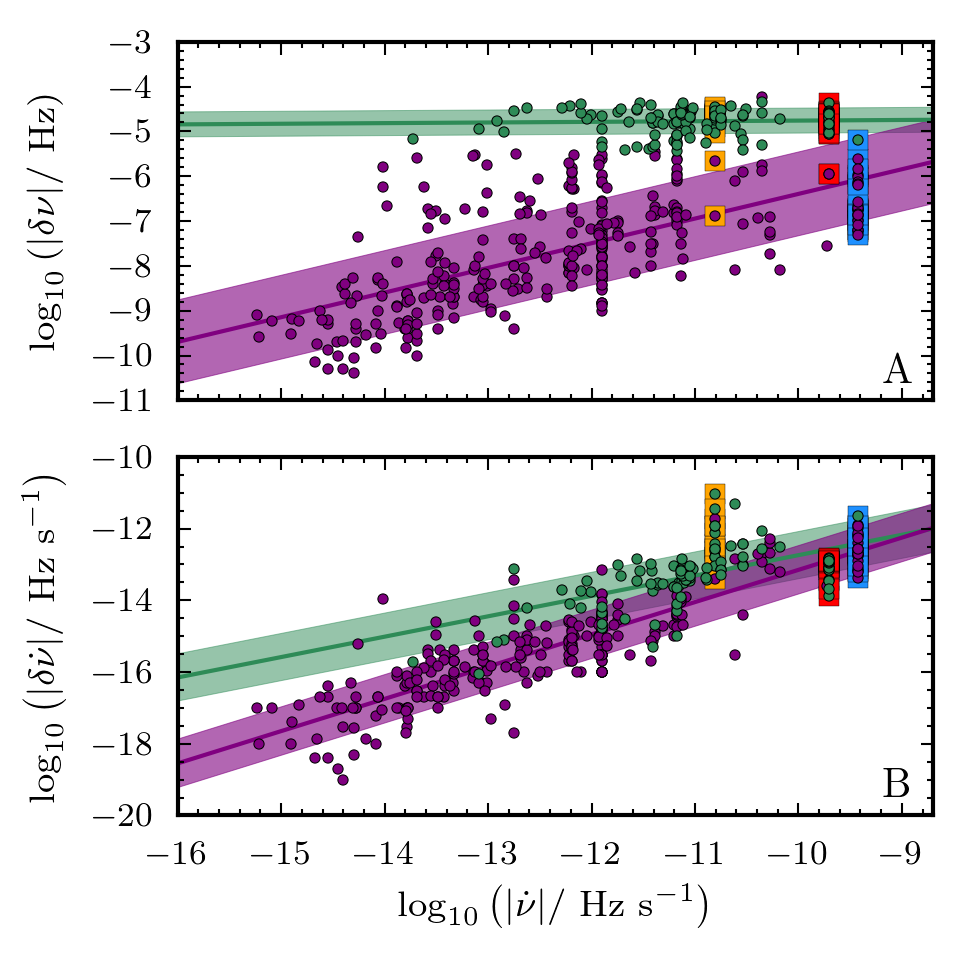
\includegraphics[width=0.75\textwidth]{Fit_Deltanu_Deltanudot}
\caption{\textbf{A}: the magnitude of $\DnuRglitch$ as a function of the source
pulsar's spin-down rate. \textbf{B}: the absolute value of the magnitude of
$\DnudotRglitch$ against the measured spin-down rate. The coloured lines and shaded
bands are the best fits from Eqn.~\eqref{eqn: Delta nu fit} for $\delta\nu$,
and Eqn.~\eqref{eqn: Delta nudot fit} for $\delta \dot{\nu}$; the green lines
mark the Vela-like fit while the purple lines park the fit to the normal population.
Vertical clustering in the observed data points is the
result of multiple glitches observed from a single source. Coloured halos
highlight glitches from some interesting pulsars.}
\label{fig: extrapolation fit}
\end{figure}

Fitting a linear function in log-log space (see Appendix~\ref{sec: linear regression in log-space} for details) our resulting fitting formulae for
the frequency jump due to each separate population is
\begin{align}
\begin{split}
\langle \DnuRglitch \rangle_{\textrm{Normal}} = &10^{-0.89}|\nudotR|^{0.55}10^{\pm0.93}
,\\
\langle \DnuRglitch \rangle_{\textrm{Vela-like}} = &10^{-4.62}|\nudotR|^{0.01}10^{\pm0.28}
.
\end{split}
\label{eqn: Delta nu fit}
\end{align}
and for the frequency-derivative jumps is
\begin{align}
\begin{split}
\langle \DnudotRglitch \rangle_{\textrm{Normal}} = &10^{-4.16}|\nudotR|^{0.90}10^{\pm0.67}
,\\
\langle \DnudotRglitch \rangle_{\textrm{Vela-like}} = &10^{-7.06}|\nudotR|^{0.57}10^{\pm0.66}
.
\end{split}
\label{eqn: Delta nudot fit}
\end{align}
Note that the last factor here provides
an estimate of the variability about the linear fit, while neglecting this term
gives the mean.
We plot both of these fitting formulae in Figure~\ref{fig: extrapolation fit};
the estimate of the variability is indicated by a shaded band.

Taking these fitting formulae, in Figure~\ref{fig: EAH Delta nu nudot prediction} we plot
the predicted glitch magnitudes (in frequency and spin-down rate respectively) over the 
S5 E@H search parameters. We have similarly
transformed the variation estimate and plotted it as a shaded band.
\begin{figure}[htb]
\centering
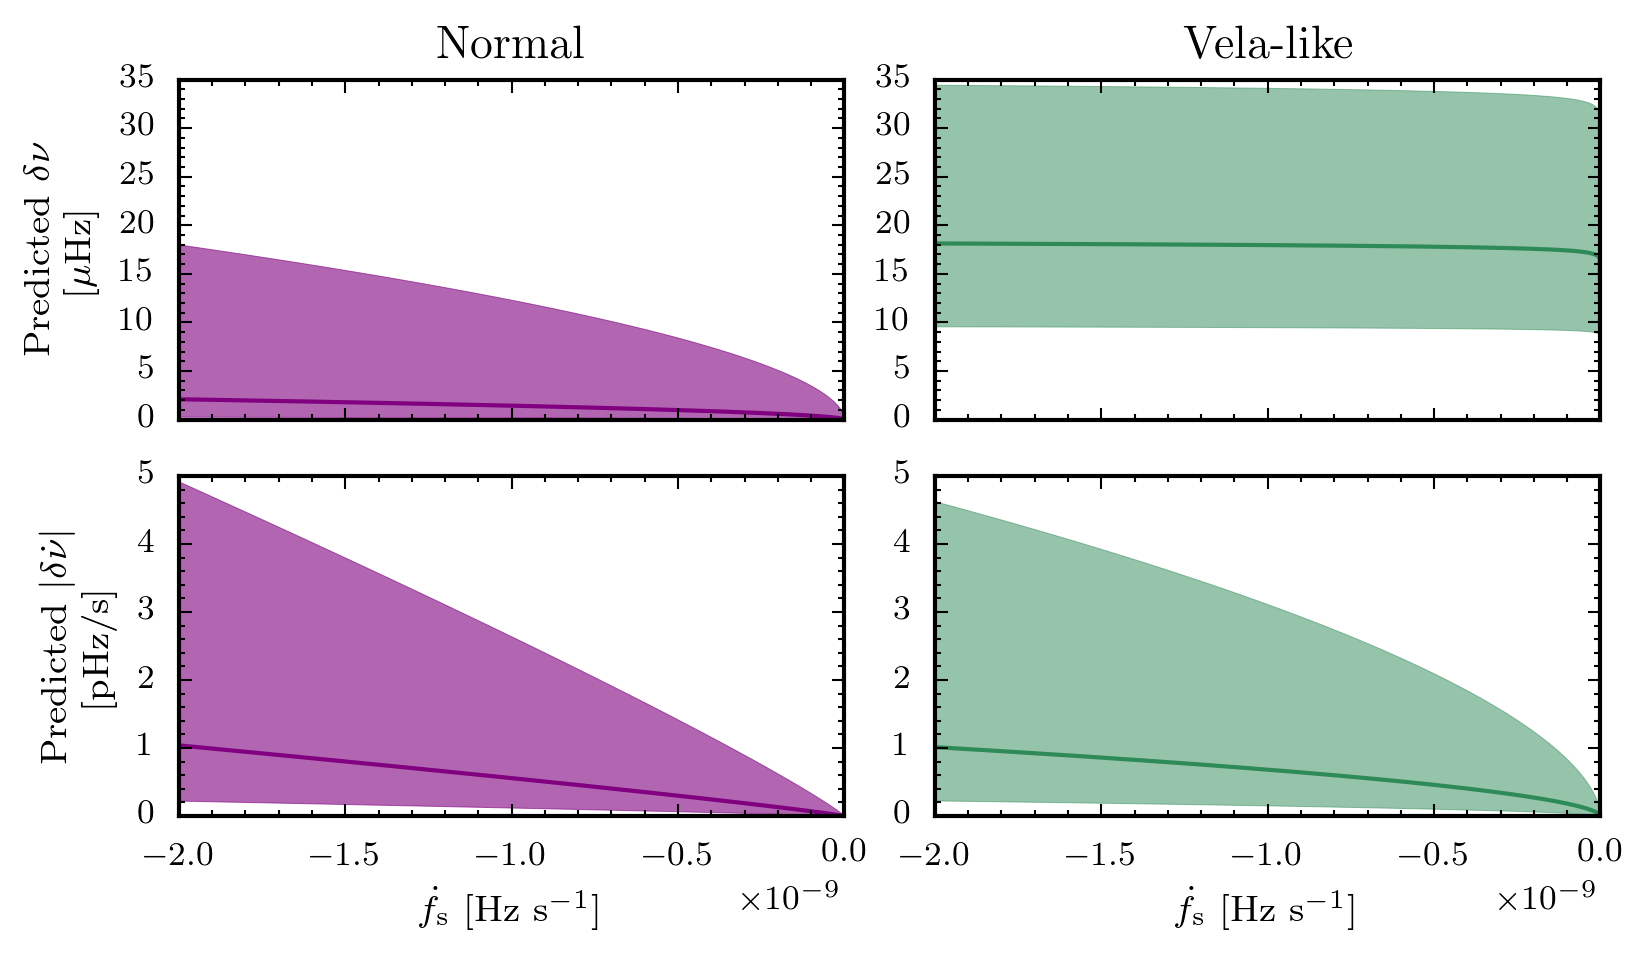
\includegraphics[]{EAH_Deltanu_Deltanudot_Prediction}
\caption{Predicted glitch magnitude of $\DnuRglitch$, in the upper panels, and
$\DnudotRglitch$, in the lower panels. These are plotted over the E@H parameter
space using the fitting formulae of Eqn.~\eqref{eqn: Delta nu fit} and
Eqn.~\eqref{eqn: Delta nudot fit}. The shaded bands indicate the estimated error
neglecting correlations.}
\label{fig: EAH Delta nu nudot prediction}
\end{figure}
These fits do not provide a precise statement about the magnitude of glitches,
but are sufficient to estimate the order-of-magnitude that we might expect.


\subsection{Extrapolating: average glitch rate}
\label{sec: average glitch frequency}
In order to estimate the average rate of glitches, \citet{Espinoza2011}
grouped pulsars by their spin-down rate $\nudotR$, including pulsars
which have not yet been observed to glitch. From this grouping, the authors
used the measured number of glitches $N_{g}$ to calculate a mean
glitch rate~$\langle \dot{N}_{g}\rangle$. In Figure~10 of their work they
show that, to a good approximation, in log-space the mean glitch rate depends linearly on the spin-down rate;
we reproduce this in Figure~\ref{fig: Espinoza 10} using the data from Table~4
of \citet{Espinoza2011}.
\begin{figure}[htb]
\centering
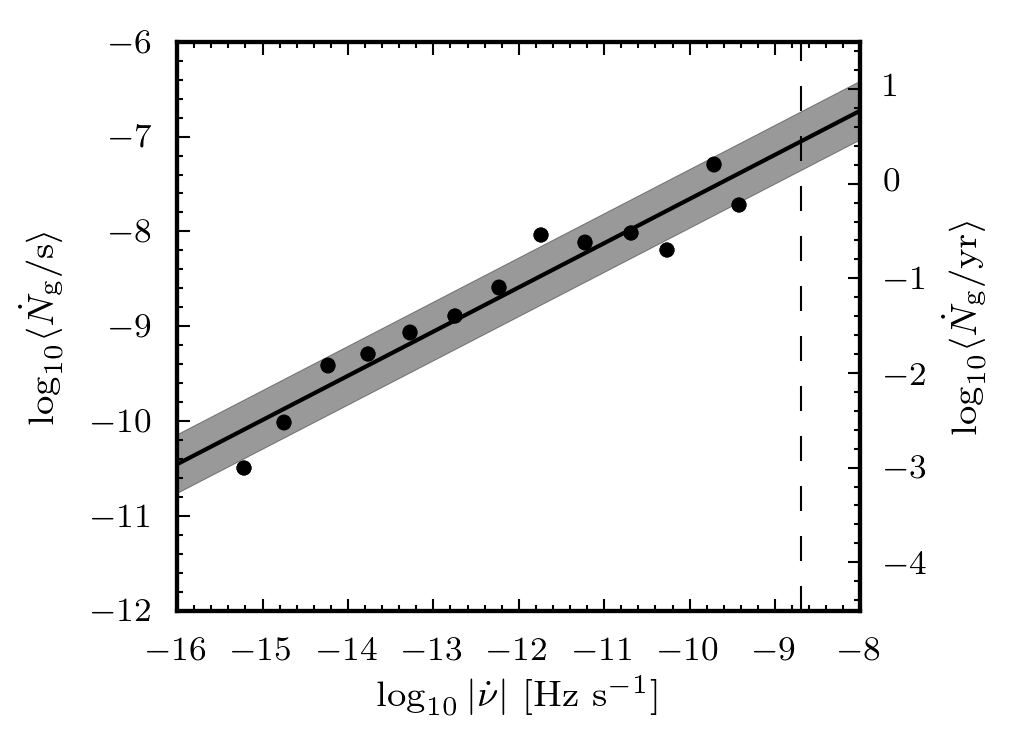
\includegraphics[width=0.75\textwidth]{Espinoza_Fig10}
\caption{Reproduction of Figure~10 from \citet{Espinoza2011} given as both log of
the glitch rate per second (left axis) and per year (right axis). Black
dots are the original data points, the solid line and shaded region are
our best-fit line and a measure of the variability as given in Eqn.~\eqref{eqn:
Ng fit}. A vertical dashed line marks $-2\times10^{-9}$, the largest absolute
spin-down rate used in the S5 E@H search.}
\label{fig: Espinoza 10}
\end{figure}

In order to extrapolate, we perform a linear regression to the data in
log-space following the method described in Appendix~\ref{sec: linear
regression in log-space}.  This gives a prediction of the glitch rate as
\begin{align}
\begin{split}
\langle \dot{N}_{\mathrm{g}} \rangle = &10^{-3.00}|\nudotR|^{0.47}10^{\pm0.31}

\textrm{ s}^{-1},
\end{split}
\label{eqn: Ng fit}
\end{align}
where $\nudotR$ is measured in Hz/s.  The exponent agrees with that found by
the original authors (they do not provide the pre-factor).

We plot this average glitch rate in Figure~\ref{fig: EAH_NdotgAve}A over the
range of $\nudotS$ values considered in the S5 E@H search. We also multiply this
rate by the span of a typical search, $\Tspan\approx1$~yr, to obtain
$\lambda(\Tspan{=}1\mathrm{yr})$, the expected number of glitches during the search; this is
also plotted in Figure~\ref{fig: EAH_NdotgAve}A, on the right-hand axis.

\begin{figure}[htb]
\centering
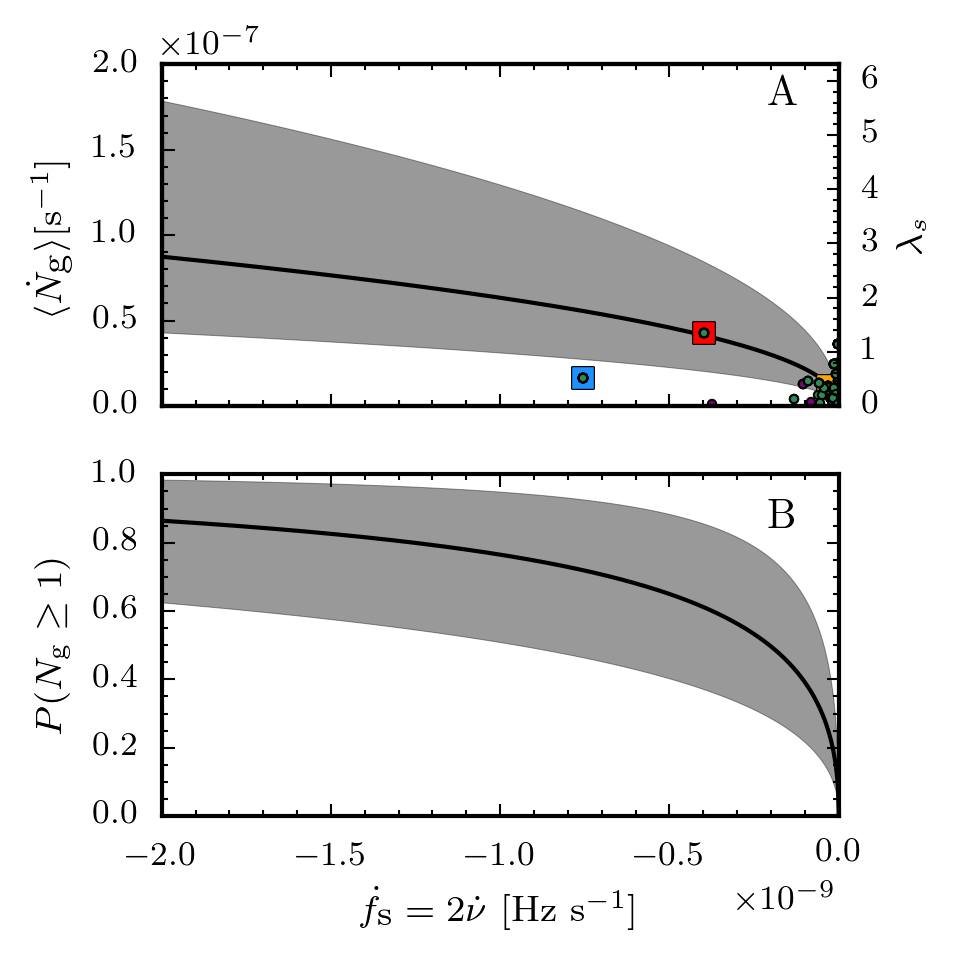
\includegraphics[width=0.75\textwidth]{EAH_NdotgAve}
\caption{\textbf{A}: the average glitch rate against the spin-down rate
$\nudotS$ over the range of values used in the S5 E@H search. On the right axis is
the corresponding average number of glitches for a search of duration $1$~yr.
\textbf{B}: the probability of observing one or
more glitches during a search lasting for $1$~yr assuming a Poisson distribution.}
\label{fig: EAH_NdotgAve}
\end{figure}

Interpreting this average glitch rate requires a substantive physical
model. \citet{Melatos2008} demonstrated that glitch waiting times are consistent
with an avalanche process transferring angular momentum from the core superfluid
to the crust. Choosing 9 pulsars which had glitched 5 times or more, they found
that 7 of these where consistent with a constant rate Poisson process such that
each glitch event is statistically independent. In the remaining two, J0537-6910
and B0833-45 (Vela), they find that a quasiperiodic component coexists with the Poisson
process and accounts for about $20\%$ of the events.

Of the glitch catalogue, J0537-6910 accounts for 23 and B0833-45 (Vela) for 17 of
the total 472 events. Assuming that $20\%$ of these are due to the
quasiperiodic component, this is $\sim 1.7\%$ of the total number of observed glitches. It
is possible that other pulsars also exhibit a quasiperiodic component, so the
total fraction of glitches from a quasiperiodic component should be greater
that $1.7\%$. However, we may still claim that the majority of glitches in the
catalogue are due to a Poisson like process.

Assuming that all glitches used to estimate $\NdotgAve$ are due to a Poisson
process, we can calculate the probability of one or more glitches occurring during
a typical search lasting $1$~yr as a function of $\nudotS$. To do this, we take the
estimated number of glitches during a typical search
$\lambda$, as given on the right axis of Figure~\ref{fig: EAH_NdotgAve}A,
and sum the Poisson probability mass function from 1 to infinity
\begin{align}
P(N_{g} \ge 1; \Tspan) = \sum_{\Ng=1}^{\infty}\frac{\lambda^{\Ng}e^{-\lambda}}{\Ng!},
\label{eqn: p one glitch or more}
\end{align}
where the dependence on $\Tspan$ is in $\lambda=\lambda(\Tspan)$.
Note that in practise we truncate the summation at a finite level where the
mass function is negligible.

In Figure~\ref{fig: EAH_NdotgAve}B we plot this probability using $\lambda$
from the upper plot. This suggests that for almost all of the E@H spin-down
rate parameter space, it is more probable to have at least one glitch per year
than to have none. This estimation will suffer bias from the inclusion of the
quasiperiodic components into the calculation of $\NdotgAve$. Nevertheless, we
hope it provides some quantitative measure of the probability of a glitch
occurring.

\section{Calculating the mismatch due to a single glitch}
\label{sec: mismatch due to glitches}

In Section~\ref{sec: statistical properties} we established the statistical
properties of observed radio pulsar glitches and provided fitting formulae for the
magnitude and rate of glitches. In this section, we will convert these
results into a quantified effect on fully-coherent and semi-coherent
GW searches using the tools developed in Section~\ref{sec: introduction to the
mismatch} and Section~\ref{sec: generalising the metric-mismatch}.

For this work, we consider a glitch to consist of an instantaneous jump in the
phase, frequency, and frequency derivative of the GW signal; the magnitudes of
these quantities we will denote by $\Dphiglitch, \Dnuglitch,$ and
$\Dnudotglitch$.  Since we don't yet understand the glitch mechanism and what
happens during the glitch, it's unclear how meaningful it is to discuss a jump
in the GW phase.  Nevertheless, modelling the signal with a piecewise Taylor
expansion naturally includes such a phase jump, therefore we will include it in
our discussion.  The size of the jump in the GW frequency and frequency
derivative can be estimated from the observed jumps in Section~\ref{sec:
statistical properties} (assuming $\Dnudotglitch = 2\DnuRglitch$ etc.). Aside
from these jumps there may also be an exponential relaxation in the post-glitch
dynamics and a rise-time during which the glitch occurs; for now all such
phenomena will be ignored, but we return to this in Section~\ref{sec: recovery}.

Our glitch signal can be modelled by a piecewise Taylor-expansion with two
subdomains. We denote the time of the glitch as $R\Tspan$ where $R$
is a dimensionless fractional quantity such that $R\in[0, 1]$ and $\Tspan$ is
the observation time of the search.
Then labelling the period before the glitch as $A$ and after as
$B$, the parameter offsets may be written
\begin{align}
\Delta\lambda^{\alpha a}(t) = \left\{
\begin{array}{lc}
\Delta\lambda^{\alpha A} & \textrm{ if } t < R\Tcoh\\
\Delta\lambda^{\alpha B} & \textrm{ if } t > R\Tcoh
\end{array}
\right.,
\label{eqn: delta lambda alpha glitch}
\end{align}
where $\dl^{\alpha j} = \ls^{\alpha j} - \lt^{\alpha j}$. We will set the
reference times for each subdomain half-way through the subdomain and also define a global
reference time $\tref$ at the glitch, $R\Tcoh$. To help orient the reader with
these choices, we provide a schematic of the signal frequency over the glitch
in Figure~\ref{fig: frequency jump}.
\begin{figure}[htb]
\centering
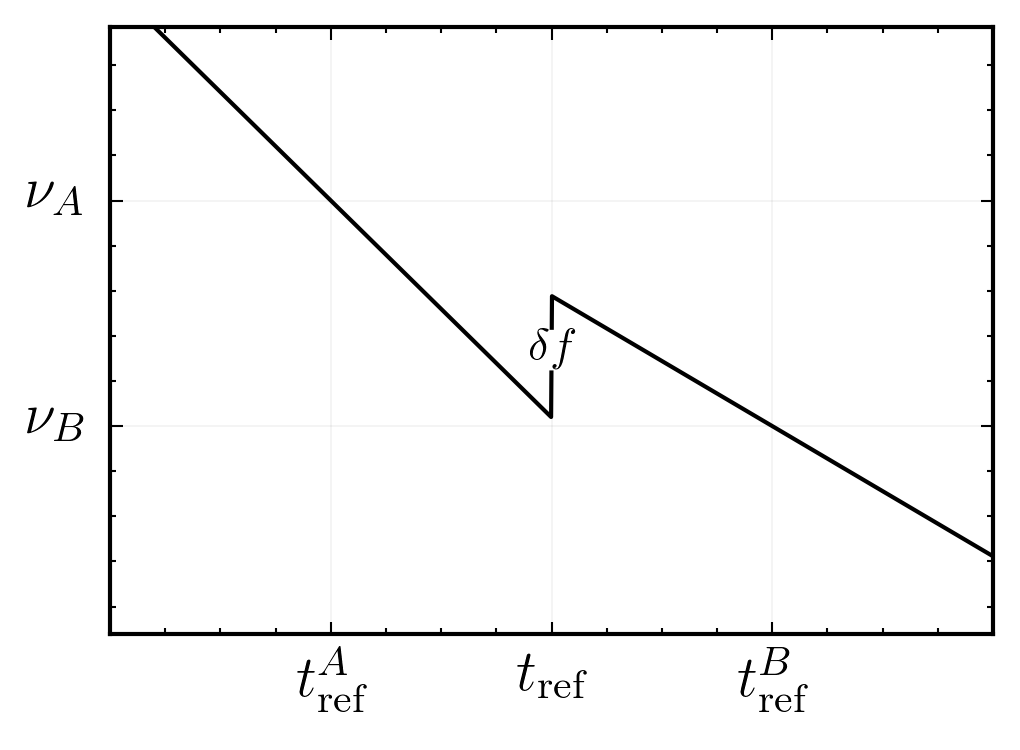
\includegraphics[]{frequency_jump}
\caption{Illustration of the references times and frequency jump over the glitch.
Note that the global reference time $\tref$ is set to coincide with the time
at which the glitch occurs; in this instant it is half-way through, but could
in general be at any time during the observation. The local reference times are
set halfway through each subdomain.}
\label{fig: frequency jump}
\end{figure}

The jumps at the glitch itself may then be parameterised as
\begin{align}
\begin{split}
\Dphiglitch & =  \phiS^{B}(R\Tcoh) - \phiS^{A}(R\Tcoh)\\
\Dnuglitch & =  \nuS^{B}(R\Tcoh) - \nuS^{A}(R\Tcoh)\\
\Dnudotglitch & =  \nudotS^{B} - \nudotS^{A}
\end{split}
\label{eqn: glitch jumps}
\end{align}
The time-dependence here indicates that one must account for the
changes due to lower order terms between the reference time, halfway through
the subdomain, and the glitch. Since we do not consider second-order spin-down
terms, this is not required for the $\Dnudotglitch$ calculation.

In the following sections, we consider fully-coherent and semi-coherent GW
searches for this signal which contains a single glitch. In general these
searches are performed over a grid of Taylor expansion templates in the
frequency and spin-down parameter space and then, if some subset of the
templates return a sufficiently high SNR, the template with the smallest
mismatch is taken as a candidate. This method minimises the mismatch with
respect to the search parameters~$\nuT$~and~$\nudotT$; we will include this
minimisation step in the calculation.

\subsection{A single glitch in a fully-coherent search}

\subsubsection{A fully-coherent search: analytic metric-mismatch}

To calculate the fully-coherent mismatch, we first expand
the summation in Eqn.~\eqref{eqn: mismatch} over the two subdomains giving three terms
\begin{align}
\begin{split}
\mutilde = &
g_{\alpha\beta AA}\Delta\lambda^{\alpha A} \Delta\lambda^{\beta A} +
2 g_{\alpha\beta AB}\Delta\lambda^{\alpha A} \Delta\lambda^{\beta B}
+ g_{\alpha\beta BB}\Delta\lambda^{\alpha B} \Delta\lambda^{\beta B}.
\end{split}
\end{align}
To calculate the metric components, we use Eqn.~\eqref{eqn: metric tref half}
with $\dT^A = R\Tcoh$ and $\dT^B = (1-R)\Tcoh$.
We then insert the parameter offsets $\Delta\lambda^{\alpha a}$
from Eqn.~\eqref{eqn: delta lambda alpha glitch},
and explicitly write the mismatch in terms of the components  of $\Delta\lambda^{\alpha a}=
[\Deltaphi^{a}, \Deltanu^{a}, \Deltanudot^{a}]$.
After some manipulation, the mismatch between the glitch signal and an arbitrary
Taylor expansion template is
\begin{align}
\begin{split}
\mutilde = & R(1-R)(\Deltaphi^A - \Deltaphi^B)^{2}
+ \frac{\pi^{2}\Tcoh^{2}}{3}
\left[R^{3}(\Deltanu^A)^{2} + (1-R)^{3}  (\Deltanu^B)^{2}\right] \\
& + \frac{\pi^{2} \Tcoh^{4}}{720}\left[
       R^{5}(9-5R)(\Deltanudot^A)^{2}
       -10R^{3}(1-R)^{3}\Deltanudot^A\Deltanudot^B
       + (1-R)^{5}(5R+4)(\Deltanudot^B)^{2}
                                       \right] \\
& + \frac{\pi \Tcoh^{2}}{6}\left[R(1-R)
    (\Deltaphi^B - \Deltaphi^A)
    ((1-R)^{2}\Deltanudot^B -  R^{2}\Deltanudot^A)
                                 \right].
\end{split}
\label{eqn: mutilde fully-coherent unminimised}
\end{align}
The first three terms are the independent contributions to the mismatch from
the jumps in phase, frequency, and spin-down; the last term is the mixture term
between the phase and the spin-down.  This expression has a maximum when $R =
1/2$, and collapses to the usual mismatch between two smooth Taylor expansions when
$R$ is 0 and 1. Furthermore, we verified that when the magnitude of the glitch
is zero, one recovers the usual fully-coherent mismatch between two smooth
Taylor expansions.

%defined in Eqn.~\eqref{eqn: parameter space offsets}
The mismatch in Eqn.~\eqref{eqn: mutilde fully-coherent unminimised} is a
function of the individual signal parameter $\ls^{\alpha a}$, and the template
parameters $\lt^{\alpha a}$. We are not interested in arbitrary choices of the template
parameters, but those which minimise the mismatch as would be found by
searching over a small area in parameter space and selecting the template with
the smallest mismatch as a detection candidate. We therefore
analytically minimise Eqn.~\eqref{eqn: mutilde fully-coherent unminimised} with
respect to the template parameters $\nuT$ and $\nudotT$.
We find that
\begin{align}
\begin{split}
\nuT^{\textrm{min}} = &
\nuS^A + \Dnuglitch(1-R)^2(2R+1)
      + \frac{3\Dphiglitch}{\pi \Tcoh}R(1-R) \\
& + \frac{\Tcoh}{2}\left(\nudotS^A(1-R)+\Dnudotglitch(1-R)^{3}(1+R)\right),
\end{split}
\end{align}
and
\begin{align}
\begin{split}
\nudotT^{\textrm{min}} = &
\nudotS^{A} + \Dnudotglitch(1-R)^{3}(6R^{2} + 3R + 1) \\
& + \frac{30\Dnuglitch}{\Tcoh} R^{2}(1-R)^{2} +
\frac{30\Dphiglitch}{\pi \Tcoh^{2}} R (1-R)(2R-1),
\end{split}
\end{align}
which are expressed at the global reference time $\tref$.

Inserting these into Eqn.~\eqref{eqn: mutilde fully-coherent unminimised} and
simplifying yields a minimum fully-coherent mismatch of
\begin{align}
\begin{split}
\mutilde = & R(1-R)(4R(1-R)(5R(1-R)-2) + 1)\Dphiglitch^{2} \\
& + \frac{\pi^{2}\Tcoh^{2}}{3} R^{3}(1-R)^{3}(4 - 15R(1-R)) \Dnuglitch^{2}\\
& + \frac{\pi^{2}\Tcoh^{4}}{5} R^{5}(1-R)^{5}\Dnudotglitch^{2} \\
& + 2\pi\Tcoh R^{2}(1-R)^{2}(1-2R)(5R(1-R)-1)\Dnuglitch\Dphiglitch\\
& + \pi^{2} \Tcoh^{3}R^{4}(1-R)^{4}(2R-1)\Dnudotglitch\Dnuglitch \\
& + \frac{\pi\Tcoh^{2}}{3}R^{3}(1-R)^{3}(2-12R(1-R))\Dphiglitch\Dnudotglitch.
\end{split}
\label{eqn: mismatch fully-coherent glitch}
\end{align}
An important distinction must be made here between $\Deltanu^{a}$ which is the
frequency offset between the signal and template in the $a^{th}$ subdomain, and $\Dnuglitch$
the signal frequency jump at the glitch. Notably, the minimum mismatch
depends only on $\DphiRglitch, \Dnuglitch$, and $\Dnudotglitch$; it is
independent of the overall phase, frequency, or spin-down of the signal.

Since the probability distribution of
$R$ should be uniform over the search duration, we can average Eqn.~\eqref{eqn:
mismatch fully-coherent glitch} over $R$ to get the expectation
\begin{align}
\langle \mutilde \rangle_{R} = &
\frac{3}{70}\Dphiglitch^{2}
+ \frac{\Tcoh^{2}}{630}\left(\pi^{2}\Dnuglitch^{2}
- \pi\Dphiglitch\Dnudotglitch\right)
+ \frac{\pi^{2}\Tcoh^{4}}{13860} \Dnudotglitch^{2}.
\label{eqn: R-averaged fully coherent}
\end{align}
The mixture terms $\Dnuglitch\Dphiglitch$ and
$\Dnuglitch\Dnudotglitch$ vanish in the averaging process.

\subsubsection{Simple estimates}

We now make some rough estimates based on Eqn.~\eqref{eqn: R-averaged
fully coherent}, the $R$-averaged mismatch for a fully-coherent search.
Firstly, let us consider a glitch which consists of a jump solely in the phase
$\Dphiglitch$. For such a glitch, we can calculate the size of a phase-jump
which would produce a mismatch of $\mutilde=0.1$
\begin{align}
\Dphiglitch =
\sqrt{\frac{70\mutilde}{3}} \approx 1.5 \textrm{ rad} \left(\frac{\mutilde}{0.1}\right)
\end{align}

For the frequency and spin-down rate jumps,
a simple way to quantify the significance of a given glitch is to ask `over
what coherence time would a fully-coherent search accumulate a mismatch of
$\mutilde=0.1$?'. We will consider each type of jump independently, since we are
only hoping to make order of magnitude estimates.
For the frequency jump we find that
\begin{align}
T_\textrm{coh} = \frac{\sqrt{630 \mutilde}}{\pi\Dnuglitch}
\approx 2.9 \textrm{ days} \left(\frac{\mutilde}{0.1}\right)^{\frac{1}{2}}
\left(\frac{\Dnuglitch}{10^{-5} \textrm{ Hz}}\right)^{-1},
\end{align}
while for the spin-down rate jump
\begin{align}
T_\textrm{coh} =
\left(\frac{13860 \mutilde}{\pi^{2}\Dnudotglitch^{2}}\right)^{\frac{1}{4}}
\approx 40 \textrm{ days} \left(\frac{\mutilde}{0.1}\right)^{\frac{1}{4}}
\left(\frac{\Dnudotglitch}{10^{-12} \textrm{ s}^{-2}}\right)^{-\frac{1}{2}}.
\end{align}
We have parameterised using the largest jumps seen in the glitch-catalogue as
can be seen in Figure~\ref{fig: Espinoza dF dF1}. This is a useful
order-of-magnitude estimate and tells us that over timescales comparable to
current and future searches (at least the fully-coherent follow-up) the
mismatch can potentially rise above 0.1.  We will investigate the predictions
of Eqn.~\eqref{eqn: R-averaged fully coherent} in depth later on in
Section~\ref{sec: estimating the mismatch}.


\subsection{A single glitch in a semi-coherent search}

Having investigated the mismatch for a glitch in a fully-coherent search, we
now consider the same glitch, but in a semi-coherent search as introduced in
Section~\ref{sec: semi-coherent mismatch}. The important
point to recall is that the semi-coherent segments must be summed along the
same point in parameter space. In practise, this means all values of the
template parameters $\lt^{\alpha}$ must be equal when expressed at the same
reference time.

\subsubsection{A semi-coherent search: analytic metric-mismatch}
\label{sec: semi-coherent searches: analytic mismatch}

For a semi-coherent search the observation time $\Tspan$ is
divided into $\Nseg$ equal length segments of duration $\Tcoh$. We then compute
the fully-coherent mismatch in each segment and then sum the squared SNR along the template
parameters to get the squared semi-coherent SNR. To calculate
the semi-coherent mismatch, we can make the simplifying assumption that the
glitch occurs exactly at the interface between two segments such that $R\Nseg$
is an integer, where $R$ measures the fraction of the observation period at
which the glitch occurs. We will derive the mismatch under this assumption and
then test how and when it breaks down using numerical simulations.

Under this assumption, in each segment both the signal and the template are
Taylor expansions and so we can use the \citet{Brady1998} formalism described
in Section~\ref{sec: the metric-mismatch approximation for fully-coherent
searches}. We do not need to use the generalised metric-mismatch developed in
Section~\ref{sec: generalising the metric-mismatch}.

For each segment we distinguish between the local reference time $\tref^j$ for
the $j^{th}$ segment and $\tref$ the global reference time, taken to be at the
glitch $R\Tspan$. Then, in the $j^{th}$ segment, the parameter offsets are calculated
by transforming the global parameters to the local offset:
\begin{align}
\Deltanu^j & = \left\{
\begin{array}{cc}
\nuT - \nuS^A + (\nudotT - \nudotS^A)(\tref^{j} - \tref)& \textrm{ if } j \le R\Nseg \\
\nuT - \nuS^B + (\nudotT - \nudotS^B)(\tref^{j} - \tref)& \textrm{ if } j \ge R\Nseg
\end{array}\right.,
\label{eqn: semi-coherent nu parameters}
\\
\Deltanudot^j &= \left\{
\begin{array}{cc}
\nudotT - \nudotS^A & \textrm{ if } j \le R\Nseg \\
\nudotT - \nudotS^B & \textrm{ if } j \ge R\Nseg
\end{array}\right.,
\label{eqn: semi-coherent nudot parameters}
\end{align}
where $\tref^{j} = \Tcoh(j - \frac{1}{2})$. We do not need to consider the
phase jump at the glitch, since the fully-coherent mismatch is insensitive
to an overall phase-offset; if the glitch did not occur
at the interface between two segments then this would not be the case.  The
template parameters $\nuT$ and $\nudotT$ are the same in each segment; this
reflects the fact that the semi-coherent search sums the SNR along a smooth
Taylor expansion template.

We calculate the metric for a fully-coherent search with the reference time
half-way through from Eqn.~\eqref{eqn: fully-coherent metric simple}; then for
the $j^{th}$ segment, we calculate the fully-coherent mismatch to be
\begin{align}
\mutilde^j = \frac{\pi^{2}\Tcoh^{2}}{3} (\Deltanu^{j})^{2}
+ \frac{\pi^{2}\Tcoh^{4}}{180}(\Deltanudot^j)^{2}
\end{align}

Inserting this into Eqn.~\eqref{eqn: semi-coherent mismatch} we average over all
the segments with the parameter offsets given by Eqn.~\eqref{eqn: semi-coherent
nu parameters} and Eqn.~\eqref{eqn: semi-coherent nudot parameters}, to calculate
the semi-coherent mismatch~$\muhat$; for brevity we do not provide the result here.

Next, we minimise $\muhat$ with respect to the global $\nuT$ and $\nudotT$ to
select the minimum mismatch. The minimising values are given by
\begin{align}
\begin{split}
\nuT^{\textrm{min}}  = & \nuS^{B}
+ \frac{R(5\Nseg^{2}(R(9-6R)-4) + 4)}{5\Nseg^{2}-4}\Dnuglitch \\
& + \frac{2R(1-R)}{5\Nseg^{2}-4}(5\Nseg^{2}R(1-R)-1)\Dnudotglitch\Tcoh,
\end{split}
\end{align}
and
\begin{align}
\begin{split}
\nudotT^{\textrm{min}} = & \nudotS^{B}
+ \frac{R(5\Nseg^{2}R(3-2R)+ 4)}{5\Nseg^{2}-4}\Dnudotglitch \\
& + 30\frac{R(1-R)\Nseg}{\Tcoh(5\Nseg^{2} - 4)}\Dnuglitch.
\end{split}
\end{align}

Inserting these back into the mismatch $\muhat$, we calculate the minimised
mismatch and express it in terms of the glitch parameters $\Dnuglitch$ and
$\Dnudotglitch$
\begin{align}
\begin{split}
\muhat = & R(R-1)\frac{5\Nseg^{2}(3R(1-R)-1) + 4}{15\Nseg^{2}-12}\pi^{2}
            \Tcoh^{2}\Dnuglitch^{2} \\
& + R(1-R)\pi^{2}\Tcoh^{4}\Dnudotglitch^{2} \\
& \hspace{5mm}\times\frac{25\Nseg^{4}R^{2}(1-R)^{2} + \Nseg^{2}(5R(R-1)-5) + 4}{225\Nseg^{2}-180} \\
& + \frac{5\Nseg^{3}R^{2}(1-R)^{2}}{15\Nseg^{2}-12}(2R-1)
   \pi^{2}\Tcoh^{3}\Dnuglitch\Dnudotglitch.
\end{split}
\label{eqn: mu semi-coherent R}
\end{align}

Assuming that the glitch should occur with the same probability at any point
during the observation, we average over $R$ and take the limit of $\Nseg$ being
large. This gives
\begin{align}
\langle\muhat\rangle_{R} = \frac{\pi^{2}\Tcoh^{2}}{45}\Dnuglitch^{2}
      + \frac{\pi^{2}\Tcoh^{2}\Tspan^{2}}{1260}\Dnudotglitch^{2}.
\label{eqn: R-averaged semi-coherent}
\end{align}
In the last step we substituted $\Nseg=\Tspan/\Tcoh$.

\subsubsection{Checking the validity of the assumption}

Eqn.~\eqref{eqn: mu semi-coherent R} relies on the assumption that the glitch
occurs exactly at the interface between two semi-coherent segments. This
assumption is valid in the limit for which $\Nseg \gg 1$, but will be imprecise
for small numbers of segments. To demonstrate this, in Figure~\ref{fig: n seg
convergence} we plot the fractional absolute difference between the $R$-averaged
metric-mismatch approximation $\langle \muhat \rangle_R$, as given in
Eqn.~\eqref{eqn: R-averaged semi-coherent}, and the $R$-averaged exact mismatch
$\left(\langle \muhat \rangle_{R}\right)_{\textrm{exact}}$ which we calculate
numerically. To test both of the terms in Eqn.~\eqref{eqn: R-averaged semi-coherent}
we plot the residual difference for two glitches: one in the frequency and
the other in the spin-down rate, the exact values are given in the legend.
\begin{figure}[htb]
\centering
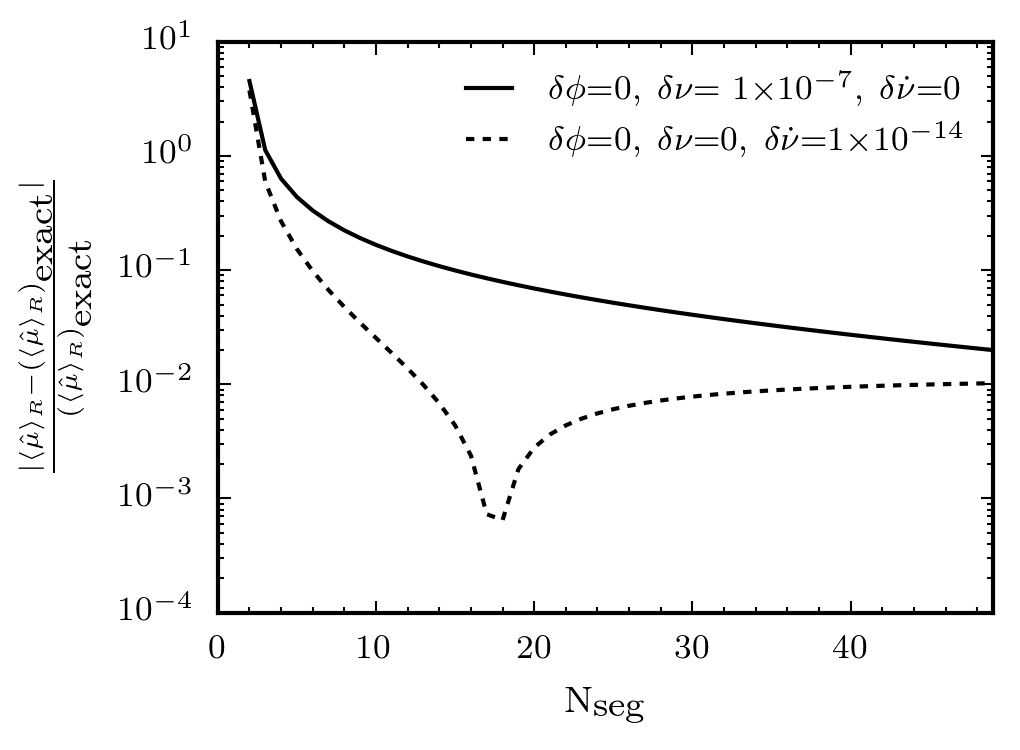
\includegraphics[]{SimulatedGlitches_NsegConvergence}
\caption{Fractional difference between the $R$-averaged
metric-mismatch approximation $\langle \muhat \rangle_R$, as given in
Eqn.~\eqref{eqn: R-averaged semi-coherent}, and the $R$-averaged exact mismatch
$\left(\langle \muhat \rangle_{R}\right)_{\textrm{exact}}$. The exact mismatch
is calculated numerically and does not suffer from either the metric-mismatch
approximation or the assumption that the glitch occurs exactly at the interface
between two segments of the semi-coherent search.}
\label{fig: n seg convergence}
\end{figure}
This figure shows that for $\Nseg > 10$ the error due to our assumption that
the glitch occurs exactly at the interface between two segments of the
semi-coherent search decreases. The error which persists for $\Nseg >> 1$ is
due to the metric-mismatch approximation which is expected and understood.

%\subsubsection{Behaviour of the semi-coherent mismatch}
%and also to
%examine the rich behaviour of Eqn.~\eqref{eqn: mu semi-coherent R}, in
%Figure~\ref{fig: varyingR} we compare the analytic result with numerical
%experiments in which the mismatch is calculated exactly. This is done for three
%triplets of $\Dnuglitch$, $\Dnudotglitch$ and $\Tspan$ chosen to show the behaviours of the
%three terms in Eqn.~\eqref{eqn: mu semi-coherent R}. For all three we use
%$\Nseg=10$ and vary $R$, the fractional point at which the glitch occurs.
%\begin{figure}[htb]
%\centering
%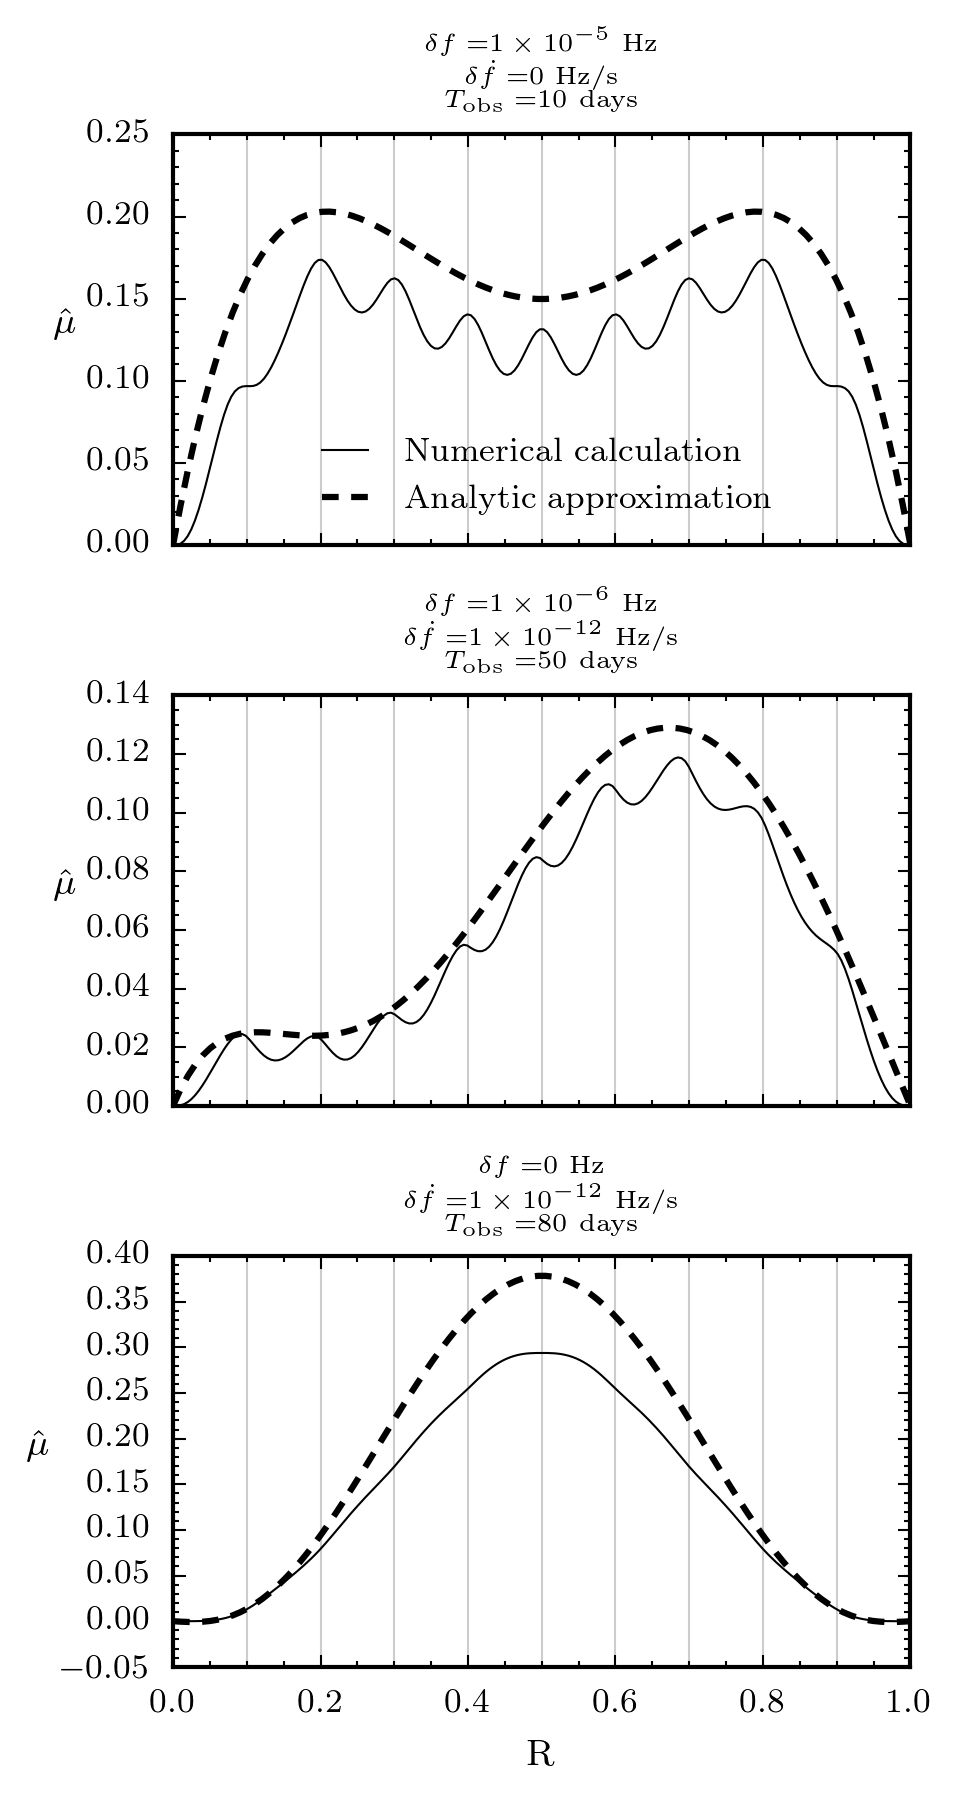
\includegraphics[]{SimulatedGlitches_VaryingR}
%\caption{Comparison of the semi-coherent mismatch as estimated by the analytic
%         approximation Eqn.~\eqref{eqn: mu semi-coherent R} with
%         exact numerical experiments for three stes of $\Dnuglitch$,
%         $\Dnudotglitch$, and $\Tspan$. For all three we use $\Nseg=10$ and add vertical bars
%         to indicate the points when the glitch occurs exactly at an interface 
%         between two semi-coherent segments.}
%\label{fig: varyingR}
%\end{figure}
%
%There are two causes of disagreement between the analytic and numerical results
%in Figure~\ref{fig: varyingR}. First, we have error due to the assumption of
%small mismatch which goes into the metric-mismatch approximation. Since the
%mismatches here are quite large $\muhat \sim 0.1$, this assumption is invalid
%and causes the analytic result to overestimate the exact numeric result. In the
%limit that $\muhat \ll 1$ when either the observation time is shorter or the
%glitch size is smaller, this source of error vanishes and the numeric and
%analytic results agree exactly, aside from the second source of disagreement.
%The second disagreement is the breakdown of the assumption that the glitch
%occurs exactly at the interface between two glitches: this is shown for all
%three plots in Figure~\ref{fig: varyingR} at point where the glitch deos not
%occur at the interface between two segments (shown as vertical lines). We have
%intentionally chosen a small number of segments,$\Nseg=10$, so that at the
%vertical lines, where $R=0.1, 0.2, \dots$, the assumption is valid and the
%analytic and numerical results will agree exactly aside from the first cause of
%disagreement mentioned above.
%
%Figure~\ref{fig: varyingR} demonstrates that Eqn.~\eqref{eqn: mu semi-coherent R}
%and hence Eqn.~\eqref{eqn: R-averaged semi-coherent} captures the essential
%features and order-of-magnitude of the semi-coherent mismatch. We will always
%use these equations in the limit that $\Nseg \ge 10$ such that the second source
%of error is negligible. The first source of error will be discussed when it is
%relevant.

\subsubsection{Simple estimates}
Taking Eqn.~\eqref{eqn: R-averaged semi-coherent}, the $R$-averaged semi-coherent
metric-mismatch,
we can estimate the maximum coherence time
for a semi-coherent search allowing for a mismatch $\mu=0.1$. For the jumps in
frequency this gives
\begin{align}
\Tcoh = \frac{\sqrt{45\muhat}}{\pi\Dnuglitch}
\approx 0.782 \;\mathrm{ days}
\left(\frac{\muhat}{0.1}\right)^{1/2}
\left(\frac{\Dnuglitch}{10^{-5}\textrm{ Hz}}\right)^{-1},
\end{align}
while for the jumps in frequency-derivative this gives
\begin{align}
\begin{split}
\Tcoh & = \frac{\sqrt{1260\muhat}}{\pi\Dnudotglitch\Tspan} \\
& \approx 0.689 \;\mathrm{ days}
\left(\frac{\muhat}{0.1}\right)^{\frac{1}{2}}
\left(\frac{\Tspan}{694 \textrm{ days}}\right)^{-1}
\left(\frac{\Dnudotglitch}{10^{-12}\textrm{ Hz}}\right)^{-1}
\end{split}
\end{align}
These values are less than the coherence time used in the S5 E@H search, which
was 25~hrs. These simple estimates therefore suggest that for the largest
observed glitches, semi-coherent searches may suffer a non-negligible mismatch.
We will investigate this and the fully-coherent mismatch case more rigorously
in the next section.

\section{Predicting the mismatch and rate of glitches in gravitational wave searches}
\label{sec: estimating the mismatch}

In this section, we will use the fitting formulae of Section~\ref{sec: observed glitch
magnitude} to predict the magnitude of glitches for a range of parameters
typical of all-sky searches. We will use the tools of Section~\ref{sec: mismatch
due to glitches} to transform the magnitudes into an estimate of the
fully-coherent and semi-coherent mismatch assuming a single glitch occurred
during the search. However, this mismatch does not give a complete picture of
the risk, since we must also consider the predicted rate of glitches.
Specifically, in converting a predicted glitch magnitude into an estimate for
the fully-coherent and semi-coherent mismatch we will make use of
Eqn.~\eqref{eqn: R-averaged fully coherent} and Eqn.~\eqref{eqn: R-averaged
semi-coherent}: the $R$-averaged mismatch assuming that a \emph{single} glitch
occurs uniformly and at random during the observation time. We can therefore
take these results as a lower bound when there is likely to be one or more
glitches. On the other hand, in regions where the chances of a glitch are low,
a large mismatch only indicates that the signal would be lost in the rare event
that a glitch had occurred. To provide the reader with both pieces of this
puzzle, we will present results on both the expected mismatch due to a single
glitch and the probability of one or more glitches occurring. This will be done
for each population of glitches separately. Let us define
\begin{align}
\lambda_{\textrm{normal}}(\dot{\nu}, \Tspan) & = w_\textrm{normal}\NdotgAve \Tspan 
\label{eqn: N normal}\\
\lambda_{\textrm{Vela-like}}(\dot{\nu}, \Tspan) & = w_\textrm{Vela-like}\NdotgAve \Tspan,
\label{eqn: N vela}
\end{align}
as the expected number of normal and Vela-like glitches where
$w_\mathrm{normal}$ and $w_\mathrm{Vela-like}$ are the weights of the two
populations as given in Table~\ref{tab: mixture components} and $\NdotgAve$ is
the fitted glitch rate as a function of $\dot{\nu}$ which is given by
Eqn.~\eqref{eqn: Ng fit}. Notice that we have made a prior specification here
that the proportion of normal and Vela-like pulsars in the target population is
the same as in the observed population. There is some evidence that in fact the
proportion of Vela-like pulsars increases with $\nudotR$; this could be
modelled by a $\nudotR$-dependent weighting, however we will ignore this effect
here. Eqn.~\eqref{eqn: N normal} and Eqn.~\eqref{eqn: N vela} can be
transformed into the probability of one glitch or more occurring during the
search by substitution into Eqn.~\eqref{eqn: p one glitch or more}. In the
following discussion it is this probability which we will report on.


%The expected (fully-coherent or semi-coherent) mismatch for a signal which may
%undergo any number of glitches during some observation span $\Tspan$ is given by
%\begin{align}
%\textrm{E}\left[\mu\right] = \sum_{i=0}^{\infty}
%P(i\textrm{ glitches})\textrm{E}\left[\mu \textrm{ for } i \textrm{ glitches}\right]
%\end{align}
%Droping the vanishing first term and recalling that the mismatch is positive,
%we can calculate a lower bound
%\begin{align}
%\textrm{E}\left[\mu\right] \ge
%P(\textrm{1 glitch})\textrm{E}\left[\mu \textrm{ for } 1 \textrm{ glitch}\right]
%\end{align}
%
%We will use the fitting formulae Eqn.~\eqref{eqn: Delta nu fit} and
%Eqn.~\eqref{eqn: Delta nudot fit} to estimate the magnitude of the glitches,
%however, in order to avoid overestimates we split these estimated by their
%population. Assuming that these two types of glitches are exhaustive, the
%expected mismatch for a single glitch is given by
%\begin{align}
%\begin{split}
%\textrm{E}\left[\mu \textrm{ for } 1 \textrm{ glitch}\right] = &
%P(\textrm{normal glitch})\E{\mu\textrm{ for 1 normal}} \\
%& +
%P(\textrm{Vela glitch})\E{\mu\textrm{ for 1 Vela}}
%\end{split}
%\end{align}
%Then expanding to conditional probabilities
%\begin{align}
%\begin{split}
%\textrm{E}&\left[\mu \textrm{ for } 1 \textrm{ glitch}\right] = \\
%& P(\textrm{normal}|\textrm{glitch})P(\textrm{glitch})\E{\mu\textrm{ for 1 normal}} \\
%& +
%P(\textrm{Vela}|\textrm{glitch})P(\textrm{glitch})\E{\mu\textrm{ for 1 Vela}}
%\end{split}
%\end{align}
%
%Calculating the probability of a glitch being Vela-like or normal requires
%a choice, since the data does not unambiguously provide such information: there
%may be some tendency for pulsars with large spindown rates to preferentially
%exhibit Vela-like glitches as discussed by \citet{Espinoza2011}, but this is
%not a well understood feature. We therefore choose to display results under
%three different choices to present the reader with the full spectrum of
%possible choices. This includes the two extreme cases where $P(\textrm{normal})=1$
%(hence $P(\textrm{Vela})=0$) and vice versa. Then we also provide a final result
%based on the prior assumption that, for the target population, the fraction of
%Vela-like and normal glitches is identical to the observed popultion. Therefore
%the probabilities are given by the weights of the two mixtures as given in
%Table~\ref{tab: mixture components}.

We note that in reality, the true mismatch for fully coherent searches will
always be bounded by $[0, 1]$, but the results of this section can exceed this
since we are using the metric-mismatch approximation. Similarly, for the
semi-coherent searches, it is in fact bounded by the minimum of $R$ and $1-R$;
this can be seen by realising that if the glitch is sufficiently large, the
minimum mismatch is achieved by fitting to the semi-coherent segments on
only one side of the glitch. Here, we
report the simpler results of naively applying Eqn.~\eqref{eqn: R-averaged
fully coherent} and Eqn.~\eqref{eqn: R-averaged semi-coherent}. The results
can therefore be interpreted by realising that if the metric-mismatch is greater than
1, there will be large true mismatch, although the exact value will depend on
where that glitch occurred during the observation span.


\subsection{Fully-coherent searches}

In this section, we present results on the expected mismatch and expected number
of glitches for fully-coherent searches. In Figure~\ref{fig: fully-coherent mismatch
Tspan} we plot contours of fixed mismatch as a function of the coherence time
$\Tcoh$ and the GW spin-down rate $\nudotS$. Alongside are plotted the number of
glitches as a function of the observation time and spin-down rate.
\begin{figure}[htb]
\centering
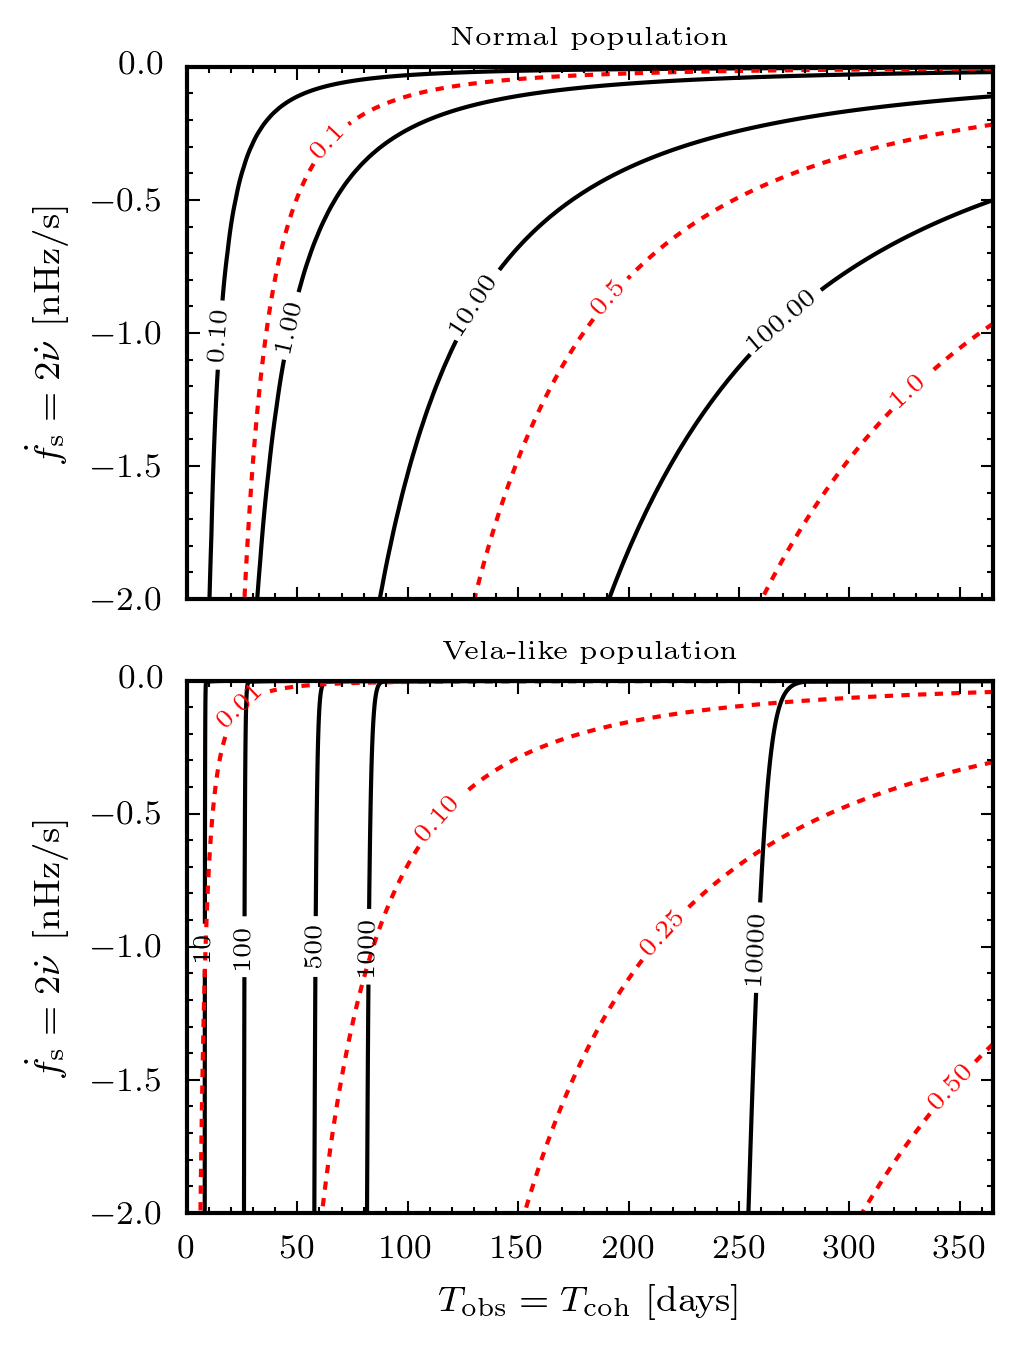
\includegraphics{fully_coherent_mismatch}
\caption{The estimated fully-coherent mismatch as a function of $\Tcoh$ and
$\nudotS$. In the top panel is the prediction based on the fit to the normal
population, in the bottom panel is the prediction based on the fit to the
Vela-like population. Solid black lines provide contours of fixed mismatch. Red
dashed lines have been added to indicate the probability (as a percentage) of
one or more normal
glitch occurring calculated by substitution of Eqn.~\eqref{eqn: N normal} (for
the normal population) or Eqn.~\eqref{eqn: N vela} (for the Vela-like
populations) into Eqn.~\eqref{eqn: p one glitch or more}.}
\label{fig: fully-coherent mismatch Tspan}
\end{figure}

These figures illustrate that the predicted mismatch depends on the source
population. For the normal population, larger absolute spin-down rates are
associated with larger glitch magnitudes; as a result larger absolute spin-down
rates are predicted to suffer more severe mismatches. For the Vela-like
population, the mismatch is largely independent of $\nudotR$, this is because
the fitting formulae Eqn.~\eqref{eqn: Delta nu fit} finds little variation in
the glitch size with the spin-down rate.

For long observation times the mismatch can be severe, however this is only a
concern if a glitch occurs. The expected number of glitches in both populations
is, for most of the parameter space, lower than 1, but not vanishingly so.

We note here that these plots only show the `best-fit' contour lines predicted
by our fitting for glitch sizes. There is substantial variability in the population
glitch sizes and rate, this is reflected in large error bars in the fitting formulae
derived in Section~\ref{sec: statistical properties}. In Appendix~\ref{sec: uncertainties}
we translate these estimates into uncertainties on the mismatch and rate
contour lines.

\subsection{Semi-coherent searches}

For the semi-coherent search we repeat the process of predicting the glitch
magnitudes, but then use Eqn.~\eqref{eqn: R-averaged semi-coherent} to
transform them into predictions for the semi-coherent mismatch. A semi-coherent search has two
fixed times: the total observation span $\Tspan$ and the coherent segment length
$\Tcoh$. In Figure~\ref{fig: semi-coherent mismatch Tspan 100} and Figure~\ref{fig:
semi-coherent mismatch Tspan 365} we present results at fixed observation times
of 100~days and 365~days and show contours of the expected semi-coherent mismatch and number
of glitches as a function of the spin-down rate and coherence time.
\begin{figure}
\centering
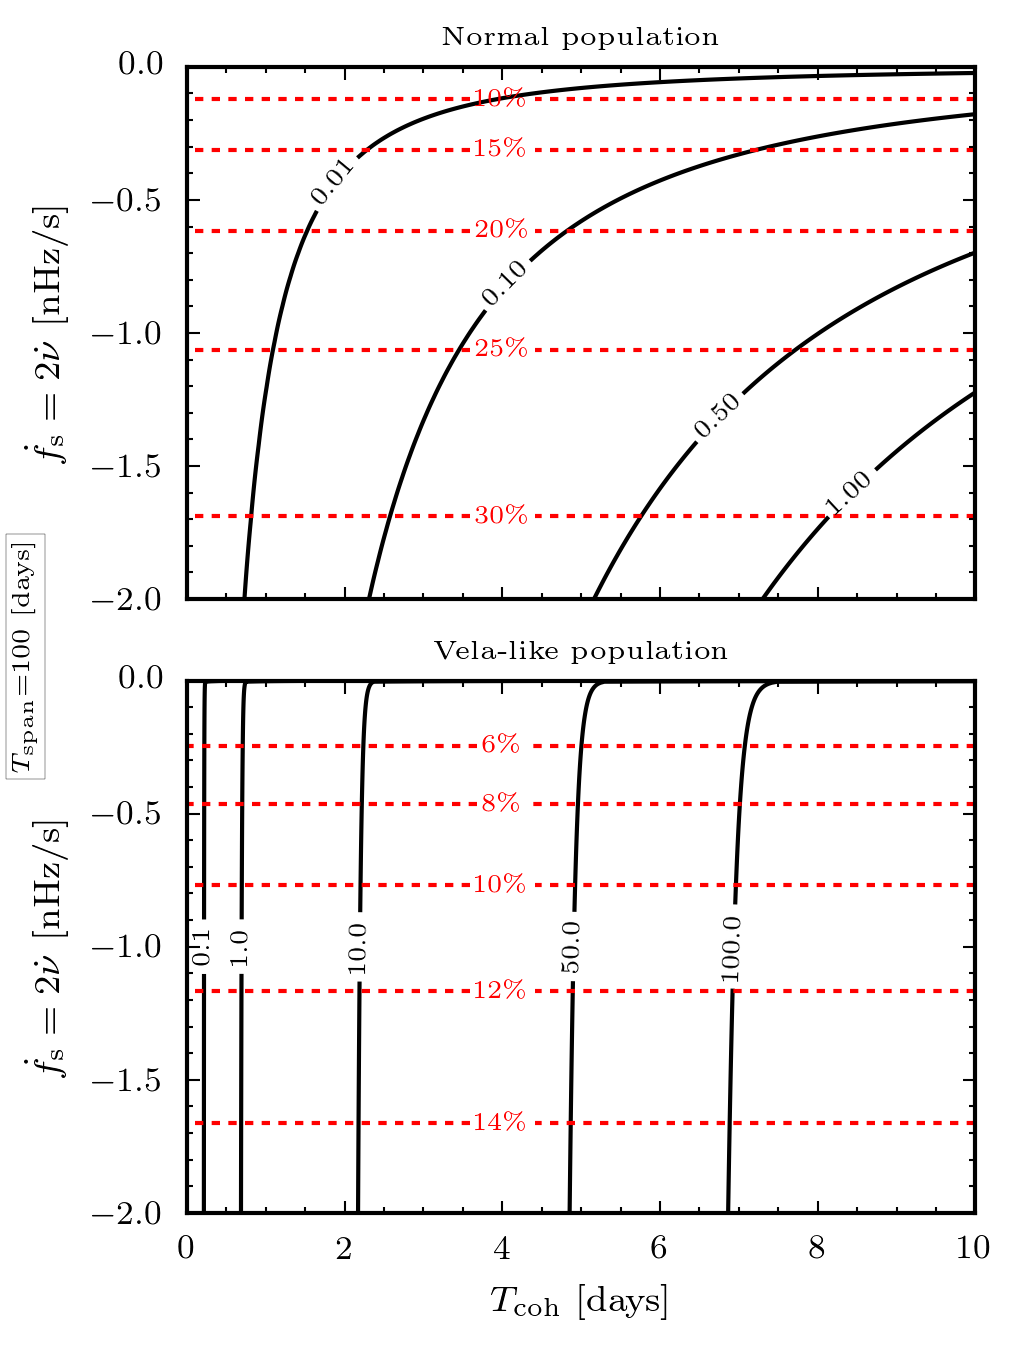
\includegraphics{semi_coherent_mismatch_Tobs_100}
\caption{
The estimated semi-coherent mismatch as a function of $\Tcoh$ and $\nudotS$ for
a fixed observation time $\Tspan=100$~days; see Figure~\ref{fig: fully-coherent
mismatch Tspan} for a description of the contour lines.}
\label{fig: semi-coherent mismatch Tspan 100}
\end{figure}
\begin{figure}
\centering
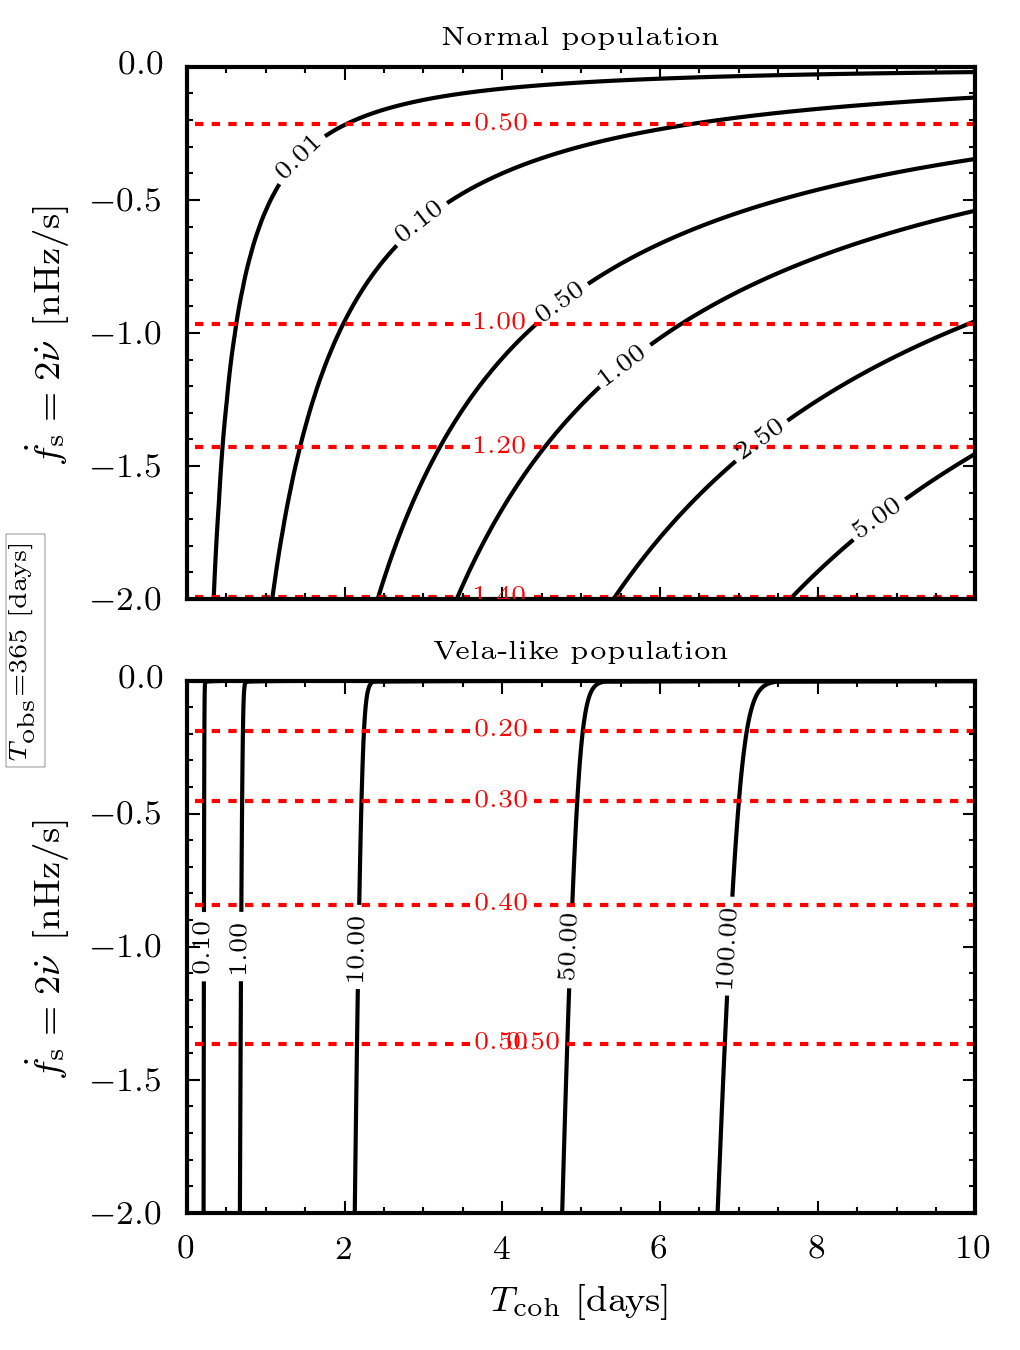
\includegraphics{semi_coherent_mismatch_Tobs_365}
\caption{
The estimated semi-coherent mismatch as a function of $\Tcoh$ and $\nudotS$ for
a fixed observation time $\Tspan=365$~days; see Figure~\ref{fig: fully-coherent
mismatch Tspan} for a description of the contour lines.}
\label{fig: semi-coherent mismatch Tspan 365}
\end{figure}

For the semi-coherent mismatch, the contour lines tell much the same story as
the fully-coherent search. The normal population produces a lower overall level of
mismatch with strong $\nudotS$ dependence while the Vela-like population has
larger mismatches with weak dependence on $\nudotS$.

As in Figure~\ref{fig: fully-coherent mismatch Tspan}, red dashed lines have
been added to indicate the probability of one or more normal glitches occurring,
this is
calculated by substitution of Eqn.~\eqref{eqn: N normal} (for the normal
population) or Eqn.~\eqref{eqn: N vela} (for the Vela-like population) into
Eqn.~\eqref{eqn: p one glitch or more}.  Note these are not a function of
$\Tcoh$ since we multiply the glitch rate per unit time by the fixed
observation period $\Tspan$.

\subsection{The follow-up stage}

A semi-coherent search begins by searching with $\Nseg$ segments to
find candidates. Following successful identification of such candidates, these
are followed-up by semi-coherent searches with fewer segments, zooming in to
constrain the parameter space. We will now show how a signal can
be identified in the initial step, but subsequently lost in the follow-up, even
if the glitch is quite small. For this exercise, we will investigate a signal
that contains a single glitch with $\Dnuglitch=5\times10^{-7}$~Hz: this is a
fairly typical normal glitch size when compared to the observed normal population (see for
example Figure~\ref{fig: Espinoza dF dF1}).

In Figure~\ref{fig: follow-up} we plot the semi-coherent mismatch for this
glitch as a function of the number of segments at a fixed observation time; this
is inversely proportional to the coherence time which we also give on the upper
axis. This is predicted
analytically from the $R$-averaged Eqn.~\eqref{eqn: R-averaged semi-coherent}.
We also performed a Monte-Carlo numerical simulation in which the mismatch was
calculated exactly for a fixed glitch size, but an $R$ chosen uniformly
throughout the observation period. The resulting mismatches are then histogrammed and the
density is shaded on to Figure~\ref{fig: follow-up}: this demonstrates the spread of
mismatches about the average value. Notably there is a tight band centred on
the analytic $R$-averaged prediction of Eqn.~\eqref{eqn: R-averaged semi-coherent};
there is a low-density of mismatches below this band. These occur when $R$ is
close to 0 or 1.

\begin{figure}[htb]
\centering
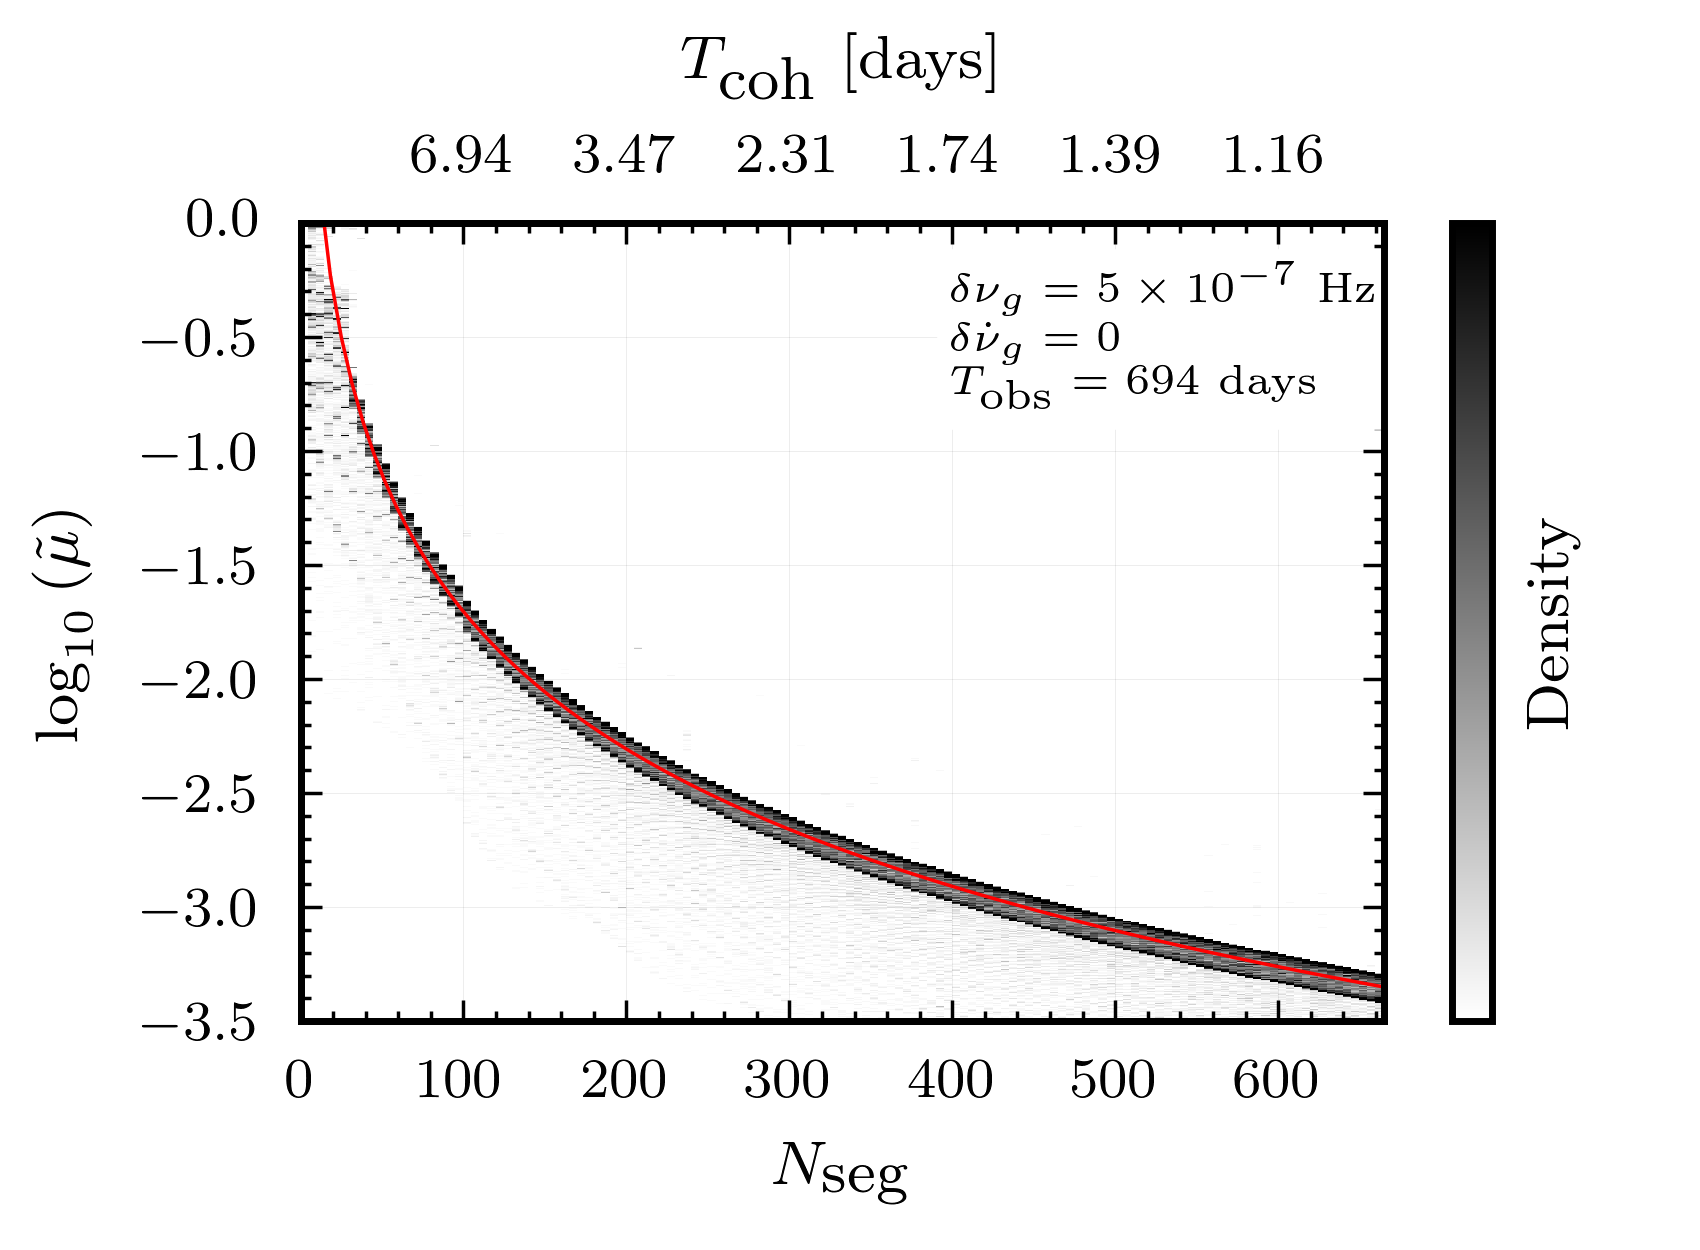
\includegraphics[width=0.75\textwidth]{S5_follow_up}
\caption{An example of how the semi-coherent mismatch changes with $\Nseg$ for
         a fixed glitch size. The red line is the prediction of the $R$-averaged
         Eqn.~\eqref{eqn: R-averaged semi-coherent}. The density map is constructed
         by performing numerical Monte-Carlo simulations over $R$ and binning the mismatches
         into histograms.}
\label{fig: follow-up}
\end{figure}
This plot shows that for this glitch during the initial search at $\Nseg=667$,
the number of segments used in the E@H all-sky search, the mismatch would be
negligible $\sim10^{-3.5}$. As a result the signal would be classified as a
candidate and subsequently followed-up. We see then that, as the number of
segments is decreased, the mismatch rapidly increases and hence the candidate
would be dismissed.

\subsection{Including the recovery from glitches}
\label{sec: recovery}
In this work, we have used the glitch catalogue maintained by \citet{Espinoza2011}
which provides $\DnuRglitch$, the instantaneous frequency increase at the
glitch. In addition to this, some glitches also undergo a short-term
exponential relaxation of some fraction of the total glitch magnitude over
times of tens to hundreds of days. \citet{Lyne2000} characterised the
fractional recovery by $Q = \sum \Deltanu_i/\DnuRglitch$ where $\sum
\Deltanu_i$ is the total glitch magnitude summed over the number of relaxation
components. For each component, $\Deltanu_i$ is recovered over an
e-folding timescale $\tau^d_i$. In most cases, only a single component is
identified.

This may have an important effect on our estimates since, if a large fraction
of the glitch is recovered in a timescale short compared to the observation
time, we will over-estimate the mismatch. On the other hand, the exponential
relaxation itself could also cause a mismatch which would tend to vanish when
$\tau^d_i \ll \Tspan$, but be maximal when $\tau^d_i \sim \Tspan$.  Ideally we would
like to model the exponential relaxation in detail, but the more practical
approach that we will take is to assume that the relaxation time is zero, such
that the actual long-term glitch magnitude is $(1-Q)\DnuRglitch$; the results in
this work can be considered to correspond to $Q=0$. The effect of this is that,
since $\mu \propto \DnuRglitch^2$, all mismatches can be rescaled by a factor
$(1-Q)^{2}$, given the size of $Q$.

To determine the appropriate size of $Q$ that we may expect, we can use the
analysis by \citet{Lyne2000}. In general, it is found that for older pulsars,
with lower spin-down rates, $Q\ll1$, but $Q$ correlates well with
$\log_{10}|\nudotR|$. Taking all measured Q values for the Crab pulsar
\citep{Lyne2000, Wang2001, Wang2012}, which has the highest spin-down rate
$-0.38$~nHz/s in the analysis, we find an average and standard-deviation of
$0.77\pm0.2$ for $Q$ and $9.45\pm6.7$~days for the relaxation timescale. We
note that in three cases the same glitch was measured with differing values of
$Q$ and relaxation time; this presumably reflects the fact that the
measurements are uncertain and depend on the data span used. In contrast, the
Vela pulsar, which has the second largest spin-down rate $0.016$~nHz/s has an
average $Q$ of 0.08 for the glitches in \citet{Lyne2000}, with none exceeding
0.2.

It is unclear what $Q$ we might expect for the target population of all-sky
searches, but we can make an estimate by taking $Q=0.8$. Given this and
assuming the relaxation time is much shorter than the observation period, this
would mean the mismatch labels of the black contour lines in Figure~\ref{fig:
fully-coherent mismatch Tspan}, Figure~\ref{fig: semi-coherent mismatch Tspan 100},
and Figure~\ref{fig: semi-coherent mismatch Tspan 365} would decrease by a factor
$\sim0.04$, ultimately meaning that longer coherence times would be more robust
to typical glitches. Nevertheless, even given this, many searches would still
be at risk to lost signals due to the presence of a glitch. These estimates are
a `best-case scenario' in that they assume $\tau^d_i =0$. A more detailed
analysis is required to understand how a recovery time which is comparable to
the observation time changes these estimate. However, it seems likely that it
will tend to increase the level of mismatch as compared to
the simple rescaling argument given here and not decrease it further.

\subsection{Application to past and future searches}
In Table~\ref{tab: past searches predictions} we present the expected number
of glitches and the metric-mismatch (normal and Vela like) for the searches listed in
Table~\ref{tab: searches}. This is done taking the \emph{worst-case} scenario
of the largest absolute spin-down rate and hence largest glitches one might
expect with no glitch recovery. Note that this is reporting the metric-mismatch
which is unbounded above: a large metric-mismatch (greater than one) indicates
a large mismatch. 
\begin{table}[htb]
\centering

\caption{Predictions for the expected number of glitches and metric-mismatch at
the \emph{highest} spin-down rates for the searches listed in Table~\ref{tab:
searches}; these are worst cases since we have chosen the highest spin-down
rates. We present results both for the number of expected glitches $\langle N
\rangle$, the fully-coherent metric-mismatch $\langle \mutilde \rangle$, and the
semi-coherent metric-mismatch $\langle \muhat \rangle$.  Note that the
supernova remnants search had no semi-coherent stage and we give the
estimate for the search for Cassiopeia A only.}

\label{tab: past searches predictions}
\tabcolsep=0.06cm
\small
\begin{tabular}{l|l|l|l|l|l|l|}
&\multicolumn{3}{|c|}{\textbf{normal population}} &\multicolumn{3}{|c|}{\textbf{Vela-like population}}\\ \hline
&$\langle N\rangle$&$\langle \tilde{\mu}\rangle$&$\langle \hat{\mu}\rangle$&$\langle N\rangle$&$\langle \tilde{\mu}\rangle$&$\langle \hat{\mu}\rangle$ \\ \hline
S5 E@H all-sky & $2.7$ & ${1.2}\times 10^{4}$ & $0.3$ & $1.2$ & ${9.0}\times 10^{4}$ & $2.7$ \\
S5 E@H galactic center & $6.2$ & ${2.6}\times 10^{5}$ & $7.2$ & $2.6$ & ${5.0}\times 10^{4}$ & $1.5$ \\
%S6 all-sky bucket & $1.1$ & $420.0$ & $0.47$ & $0.48$ & ${1.0}\times 10^{4}$ & $14.0$ \\
S5 all-sky & $0.98$ & $260.0$ & ${9.8}\times 10^{-6}$ & $0.42$ & ${2.0}\times 10^{4}$ & ${9.2}\times 10^{-4}$ \\
VSR low-frequency all-sky & $1.5$ & ${1.2}\times 10^{3}$ & ${3.8}\times 10^{-3}$ & $0.65$ & ${5.9}\times 10^{3}$ & ${2.2}\times 10^{-2}$ \\
S5 supernova remnant (Cas A) & $0.16$ & $3.0$ & $-$ & ${6.8}\times 10^{-2}$ & $12.0$ & $-$ \\
%O1 E@H all-sky & $0.82$ & $140.0$ & $3.7$ & $0.35$ & ${5.3}\times 10^{3}$ & $170.0$ 

\end{tabular}
\end{table}

This table gives a clear picture that for all searches in the fully-coherent
follow-up, the worst mismatches are greater than one. It is true that the probability
of a glitch is less than one, but not by a sufficient margin to consider them
unaffected. However, the mismatch in the semi-coherent stage can be sufficiently
small to be immune to glitches, provided the coherence times and observation
times are small enough.

\section{Conclusions}
\label{sec: conclusion}

We have investigated the effects of glitches in the GW signal when searched for
using semi-coherent and fully-coherent matched filtering techniques.

In Section~\ref{sec: statistical properties} we confirmed the observation by
\citet{Espinoza2011} that glitches can be regarded as originating from two
distinct populations named Vela-like and normal, with the Vela-like undergoing
larger glitches. We then separated the data according to their predicted source
population and found fitting formulae for the glitches magnitudes using the
spin-down rate $\nudotR$ as a predictor variable. Separating the populations
was necessary to avoid overestimating the glitch magnitudes when
extrapolating into the parameter space of all-sky gravitational wave searches where few pulsars
have been observed. We then used fitting formulae based on data from
\citet{Espinoza2011} to investigate the rate of glitches.

In Section~\ref{sec: mismatch due to glitches} we calculated the metric-mismatch for a
glitch with no exponential relation. This was done both for a
fully-coherent and semi-coherent searches (Eqn.~\eqref{eqn: R-averaged fully
coherent} and Eqn.~\eqref{eqn: R-averaged semi-coherent} respectively) assuming
that a single glitch occurs during the search. For each type of search, we provided
some simple estimates of the mismatch for the largest glitches seen in the
glitch catalogue.

Finally, we transformed our fits for the glitch magnitudes in the EM channel
into predictions for the continuous GW channel assuming that $\nuS=2\nuR$. This
prediction for the glitch magnitude was then used to estimate the mismatch for
typical search durations. This predicts that in the initial semi-coherent
search, a single glitch will cause a moderate level of mismatch if either the glitch
is Vela-like, or normal with the neutron star having a large absolute spin-down
rate. If a candidate signal with a glitch does get captured in the
semi-coherent stage, we show that, if naively followed up by a single
fully-coherent search over the full observation time, it will most likely have
a mismatch greater than 10\% unless it has a very low absolute spin-down rate.
These calculations assume that a single glitch occurred during the search. To
complete the picture, we used our fitting formulae for the expected number of
glitches to show that for typical search durations there is a reasonable chance
that a glitch will occur.

The mismatch estimates potentially overestimate the effect by ignoring
the exponential recovery from glitches. If these have short recovery timescales
compared with typical observation times, this could reduce the mismatch by a
factor of $(1-Q)^{2}$, where $Q$ is the glitch recovery parameter. It's unclear
exactly what value $Q$ should take for the target population, but we feel this
is unlikely, even in the most optimistic scenarios, to nullify the risk.

The levels of mismatch measured here are of concern to both future and past
all-sky searches for continuous GWs from neutron stars. If the effect of
glitches is ignored, detectable signals could easily by missed due to the
presence of a glitch. In a fully-coherent search the presence of a glitch can
easily be determined either by including it as a search parameter, or by
considering different sections of data. A glitch has a weaker effect on a
semi-coherent search and so it is possible the signal will be identified as a
candidate, but subsequently lost in the follow-up.  We therefore recommend
modifying follow-up procedures by introducing a greater number of steps. By
studying how the mismatch increases with the coherence time candidates when a
glitch can be identified and followed up using a search template which includes
a glitch.

%\section{Acknowledgements}
%We kindly thank Christobal Espinoza for advice on working with the glitch
%catalogue.

\begin{subappendices}
\section{Bayesian model comparison: test of mixture models}
\label{sec: Bayesian model comparison}

It seems clear by eye that the histogrammed magnitudes of the frequency change
in a glitch, $\log_{10}|\DnuRglitch|$, as shown in Fig.~\ref{fig: Delta nu
mixture}, exhibit at least two distinct modes,
which suggests that it is generated by more than one
mechanism. To model this, we will use a Gaussian mixture model (GMM)
\citep{gelman2013bayesian} with $N$ components. This model assumes that the
measured data is taken from a population with $N$ sub-populations, each having
a Gaussian distribution with separate mean, variance and weight
($\mu_{i}$, $\sigma^{2}_{i}$, $\lambda_{i}$) where $i \in [1, N]$; note that $\sum_{1}^{N} \lambda_{i} = 1$.
Furthermore, we can also allow each of the components to be
skewed with a dimensionless skew parameter $\alpha_i$ which can be either
positive or negative determining the direction of the skew, or 0, for which
there is no skew. Following \citet{Ohagan1976} then
the probability density function of the $i^{th}$ skewed Gaussian component is
\begin{equation}
f(x; \mu_i, \sigma_i, \alpha_i)
= 2 \mathcal{N}(x; \mu_i, \sigma_i)
\int_{-\inf}^{x} \mathcal{N}(\alpha_i x; \mu_i, \sigma_i) dx,
\end{equation}
where $\mathcal{N}$ denotes the Gaussian distribution.

Let $y_{i}$ be the measured values of $\log_{10}|\DnuRglitch|$
and $\vartheta$ be the collection of all model parameters
$\{\mu_i, \sigma_i, \alpha_i, \lambda_i\}$.
Then the probability density for a GMM with $N$ components is
\begin{align}
P(y_i| \textrm{model}, \vartheta) =
 \sum_{i=1}^{N} \lambda_i f (y_i; \mu_i, \sigma_i, \alpha_i).
\end{align}

To compare different choices of $N$, we will perform a Bayesian model
comparison (see \S 4.2 of \citet{jaynes2003probability} for an introduction)
between each of the mixture models and the simplest hypothesis, a mixture model
with N=1.

\newcommand{\yave}{\langle y \rangle}
\newcommand{\yran}{| y |}
\newcommand{\ystd}{\textrm{std}(y)}
For each model parameter we must specify a prior. We list these in
Eqn.~\eqref{eqn: prior} having defined $\yave, \yran$, and $\ystd$ as the average,
range, and standard-deviation of the data.
\begin{align}
\begin{split}
P(\mu_i) & = \textrm{Unif}(\yave - \yran, \yave + \yran), \\
P(\sigma_i)  &= \textrm{Half-Cauchy}\left(0, \ystd\right), \\
P(\lambda_i)  &= \textrm{Unif}(0, 1), \\
P(\alpha_i)  &= \mathcal{N}(0, 10\times\ystd).
\end{split}
\label{eqn: prior}
\end{align}
For the mean $\mu_i$ we use a uniform prior over a range of values containing
all data points.  For the standard-deviation $\sigma_i$, we will use a
Half-Cauchy distribution with zero-mean as suggested by
\citet{gelman2006prior}. A large standard-deviation, as compared to the
standard deviation of the data itself, provides a weakly informative prior.
Instead, we use a standard deviation of $\frac{\ystd}{2}$ to favour GMM
components with small standard-deviations as compared to the data. That is, our
prior disfavours models in which any of the components are wide and flat. The
prior for $\lambda_i$ is uniform on $[0, 1]$ and for $\alpha_i$ is normally
distributed with zero mean and a wide, weakly-informative standard deviation.
The choice of a zero mean favours non-skewed components. Note that, the
non-skewed models do not include $\alpha_i$ as a model parameter and the GMM
with $N=1$ does not include $\lambda_i$.

We use this choice of prior for the model parameters of each component in the
GMM with $N$ components.  In this way, models with larger values of $N$ have a
larger `prior volume' and hence there is a natural Occam-factor favouring the
simpler models with fewer components; this prevents over-fitting.

We will present results for the Bayes factor between a GMM with $N$ components
and the simplest model, a GMM with $N=1$  components. This is computed by
\begin{align}
\frac{P(\textrm{model}| \{y_i\})}{P(N=1|\{y_i\})} & =
\frac{\int_{\theta}P(\{y_i\}| \textrm{N GMM}) P(\theta) d\theta}
{\int_{\vartheta}P(\{y_i\} | \textrm{N=1 GMM}) P(\vartheta) d\vartheta}.
\end{align}

We use the \emph{emcee} \citep{Foreman-Mackay2013} MCMC algorithm to sample from the
posterior and thermodynamic integration to estimate the evidence integrals
\citep{Goggans2004}. In Table~\ref{tab: BF} we provide the $\log_{10}$ of the
Bayes factor for several possible models.
\begin{table}[htb]
\centering
\begin{tabular}{l|c}
model & $\log_{10}\left(
\frac{P(\textrm{model}| \mathbf{d})}{P(\textrm{N=1 GMM}| \mathbf{d})}
\right)$ \\ \hline
2-components & 39.12 $\pm$ 0.19 \\ 
2-components (skewed) & 41.60 $\pm$ 0.21 \\ 
3-components & 42.70 $\pm$ 0.23 \\ 
4-components & 44.27 $\pm$ 0.24 \\ 
5-components & 44.18 $\pm$ 0.22 \\ 
6-components & 43.21 $\pm$ 0.22 \\ 
7-components & 42.26 $\pm$ 0.22 \\ 

\end{tabular}
\caption{Table of the Bayes-Factor for all models considered in this study
compared to the simplest N=1 GMM. The error is an estimate of the numerical
error in the thermodynamic integration. }
\label{tab: BF}
\end{table}
The Bayes factor between any two of the models given in Table~\ref{tab: BF} can
be calculated from their difference.

This table clearly shows that the data is decisive: a Gaussian mixture model
with $N \ge 2$ fits the data a great deal better than the simple $N=1$ GMM.
This is unsurprising given the distinct multimodal nature of the data.
However, the differences between the other models is more subtle. No single model
distinguishes itself by a decisive odds-ratio compared to its neighbouring
models. We
have checked that these results are robust to small changes in the prior
specification.

To help illustrate the differences between some of these models, in Figure~\ref{fig: pdf}
we plot the probability density for the maximum posterior model parameters
found for each model.
\begin{figure}[htb]
\centering
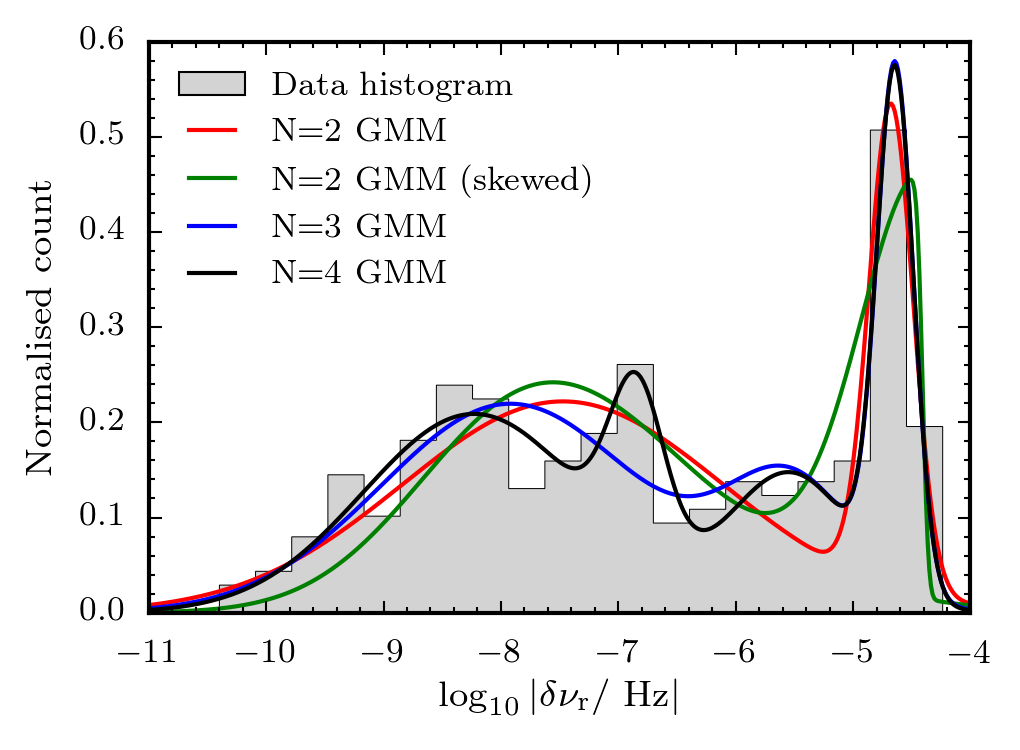
\includegraphics[width=0.5\textwidth]{GMM_comparison}
\caption{The distribution of glitch sizes in frequency along with the predictions
         for the components of several GMM. The Bayes-factor for these models
         can be found in Table~\ref{tab: BF}.}
\label{fig: pdf}
\end{figure}
It is clear from these plots that the $N=2$ model is not perfect, especially in predicting
the number of glitches found in between the two primary subpopulations,
around $\log_{10}|\DnuRglitch/\textrm{Hz}|=-5.5$; by comparison the
$N>2$ models and the $N=2$ model which allows for skewness can explain these
points and this is reflected in the Bayes factor.

From this analysis it is difficult to decide which model best fits the data. However,
what is clear is that simply modelling the data as a GMM with two components with
a skew provides a reasonable empirical model. For this reason, in our analysis of the
glitch population we will use this model and not any of the
models with a greater number of components.

It is important to realise that this comparison is purely
empirical, in that the result was not conditioned on a substantive physical
model. It would be interesting to include such modelling, this may provide some
insight into the appropriateness of the mixture model and the number of
components.

\section{Linear regression in log-space}
\label{sec: linear regression in log-space}
In Section~\ref{sec: statistical properties} we perform several linear regressions
in log-space in order to calculate power-law fits. This assumes that the observed
values $\log(y_i)$ depend on the predictor values $\log(x_{i})$ as
\begin{align}
\log(y_i) = m \log(x_i) + c + \epsilon_i
\label{eqn: linear regression}
\end{align}
where the $\epsilon_i$ are independent and
identically central normally  distributed variables with a standard-deviation $\sigma$.
In this way, $m$ and $c$ are the linear fit free variables, while $\sigma$ is
a measure of the variability in the observation about this linear fit.

We use a Bayesian linear regression in which we estimate the posterior distributions
of all three parameters using a Markov chain Monte Carlo algorithm; for the prior
distributions we use non-informative priors and test that these do not induce
any bias. In all cases we find the resulting posteriors to be Gaussian and so
can take their mean values to get best-fit parameters.
The advantage of this
method compared to a simple least-squares linear regression is that we also estimate
$\langle\sigma\rangle$, the variation about the linear fit. The linear fit can
therefore be written as
\begin{align}
y(x) = \langle m \rangle x + \langle c \rangle \pm \langle \sigma \rangle
\end{align}
We can then rearrange this equation to give the corresponding power law fit
in linear space
\begin{align}
y(x) = 10^{\langle c\rangle}x^{\langle m \rangle} 10^{\pm \langle\sigma\rangle}
\end{align}
where the last term gives the variability about the mean. Hence neglecting
this term gives the mean.

This is an inherently problematic approach since many functions besides a
power law can appear linear in a log-log plot and the assumption of
Gaussian error itself may not be valid. Nevertheless, we will still apply this
approach since we need only order-of-magnitude estimates and can always check
our predictions; we must be clear that the power-law fit gives a good empirical
fit, but is not intended to signify any substantive underlying model.


\section{Understanding the uncertainty in the predictions}
\label{sec: uncertainties}

As with all prediction, our estimates carry uncertainties both in the process
itself, and in the spread of the observed population. In calculating the
expected mismatch, the biggest source of errors come from the variability in
the size of glitches in both $\DnuRglitch$ and $\DnudotRglitch$, as shown by the
shaded bands plotted in Figure~\ref{fig: extrapolation fit}.
\begin{figure}[htb]
\centering
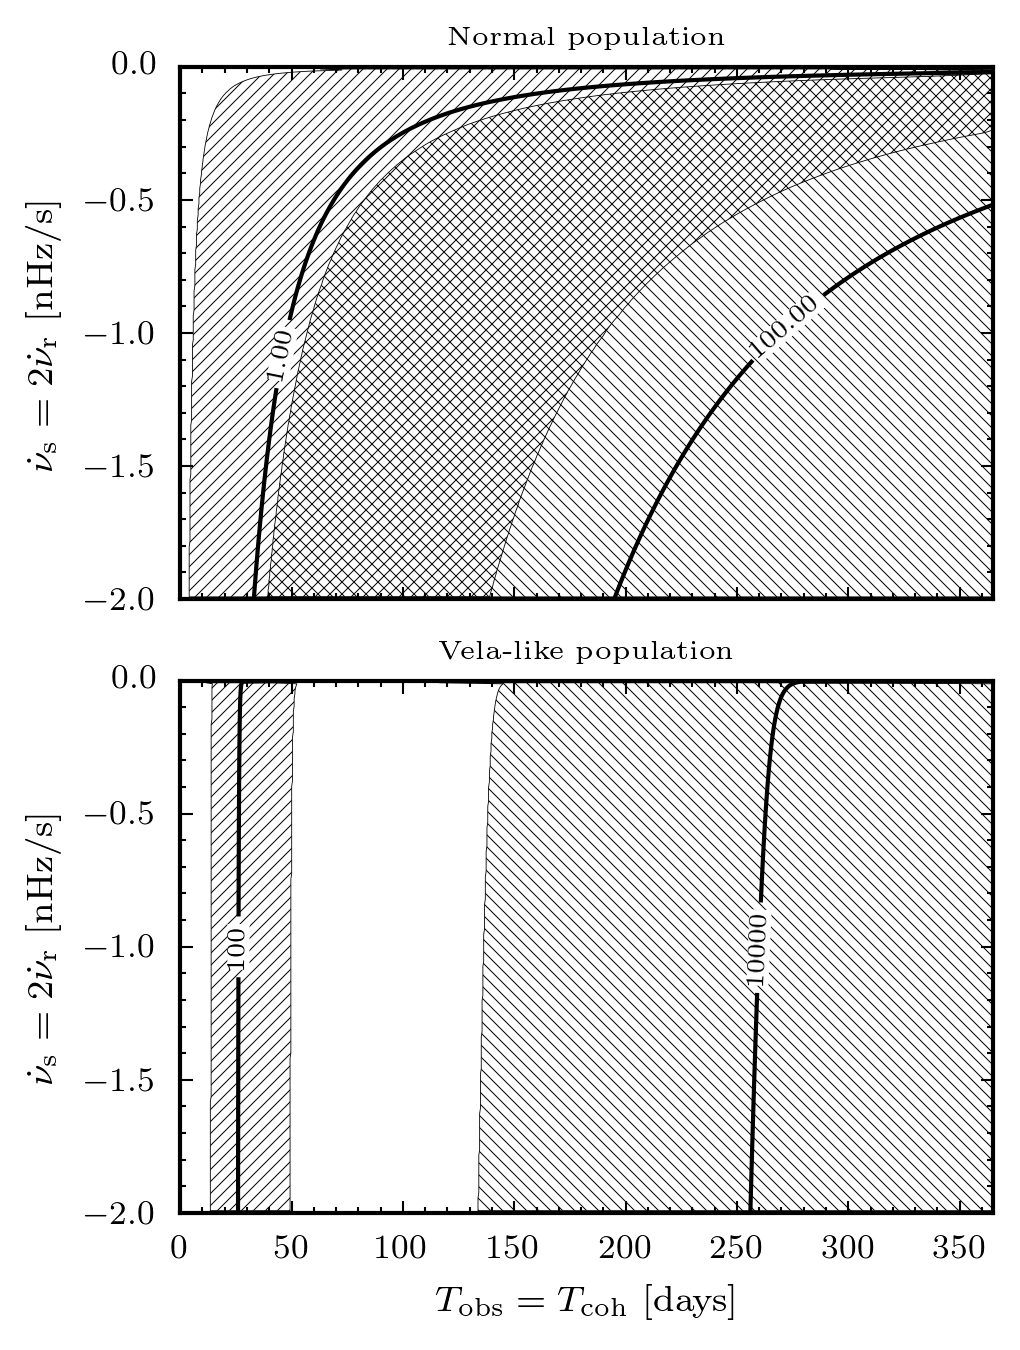
\includegraphics{fully_coherent_mismatch_errors}
\caption{A reproduction of the mismatch contours in Figure~\ref{fig:
fully-coherent mismatch Tspan} with a
reduced number of contours, but showing the variation in predicted mismatch
due to the $1\sigma$ uncertainty in the predicted distributions as given by
the shaded bands in Figure~\ref{fig: extrapolation fit}. The two uncertainty
bands overlap, giving rise to the cross-hatched region.}
\label{fig: fully-coherent mismatch Tspan errors}
\end{figure}
Also, calculating the expected number of glitches we have
uncertainty from the variability as shown by the shaded bands in Figure~\ref{fig:
Espinoza 10}. To understand how these uncertainties may change our belief in
the conclusions, in Figure~\ref{fig: fully-coherent mismatch Tspan errors} we have
repeated the analysis that led to Figure~\ref{fig: fully-coherent mismatch Tspan},
with a reduced number of
contour lines, and propagated the measure of uncertainty in the glitch sizes.
Specifically, we fill contour lines between the uncertainties in the mismatch, given by
the error in Eqn.~\eqref{eqn: Delta nu fit} and
Eqn.~\eqref{eqn: Delta nudot fit}.
\begin{figure}[htb]
\centering
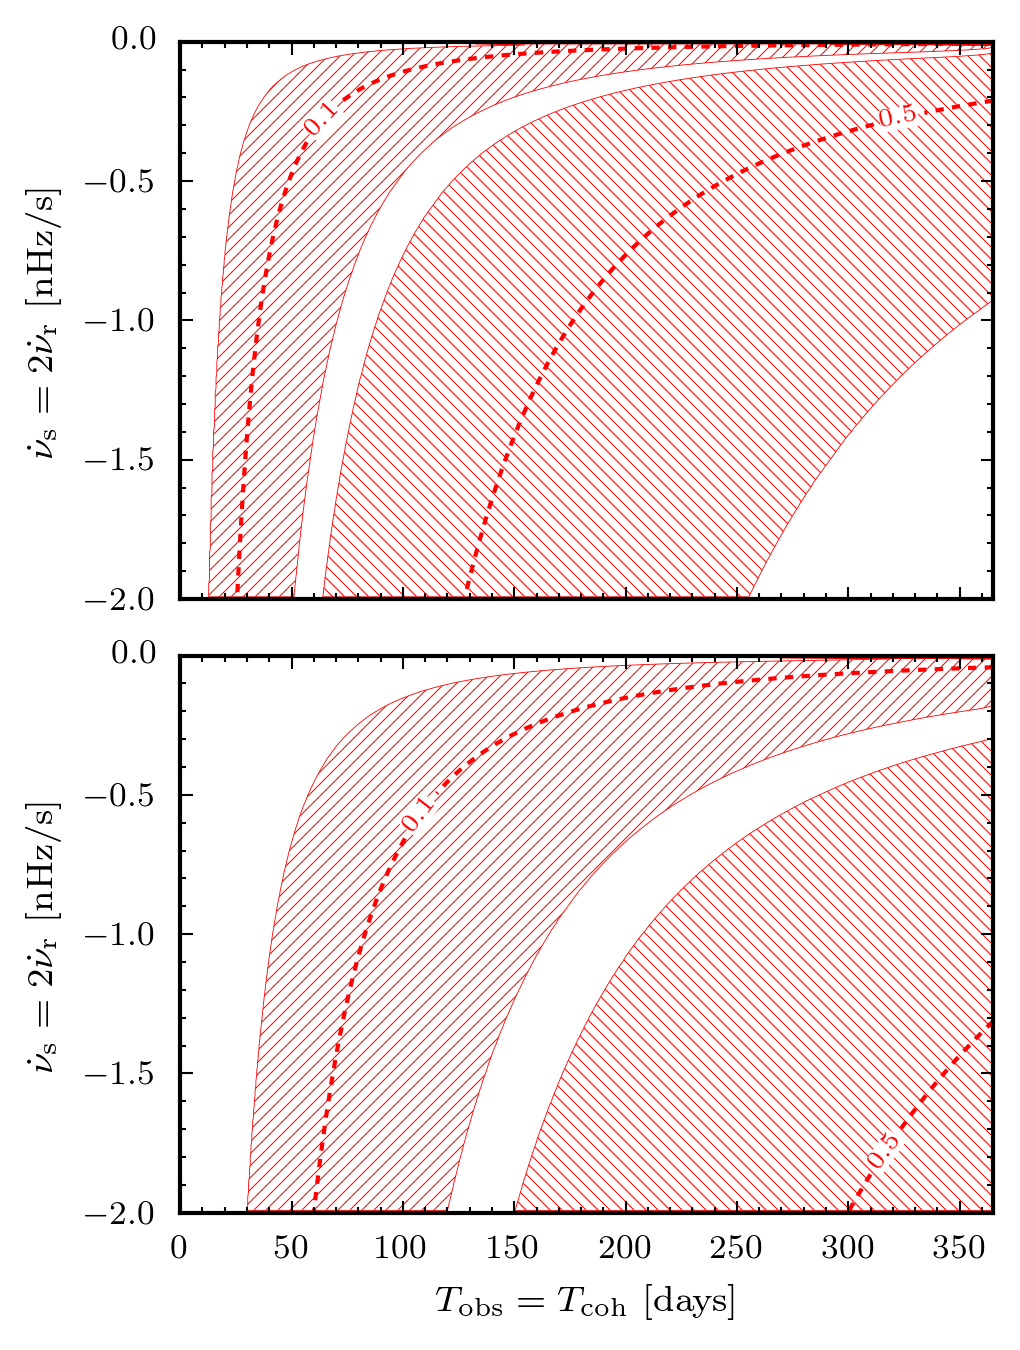
\includegraphics{fully_coherent_number_errors}
\caption{A reproduction of the number of glitches in Figure~\ref{fig:
fully-coherent mismatch Tspan} with a
reduced number of contours, but showing the variation in the expected number
of glitches due to the uncertainty in the glitch rate fit of Eqn.~\eqref{eqn:
Ng fit}.}
\label{fig: fully-coherent number Tspan errors}
\end{figure}
In Figure~\ref{fig: fully-coherent number Tspan errors}
we repeat the exercise showing the uncertainty on the number of glitches as
given by the error in Eqn.~\eqref{eqn: Ng fit}.

These figures illustrate that our uncertainty in exactly where the contour lines
sit is large. Nevertheless, even in the best case scenarios large portions of the
parameter space remain at risk.
\end{subappendices}

\biblio

\end{document}
